\documentclass{report}
\usepackage[utf8]{inputenc}
\setlength{\parindent}{0em}
\setlength{\parskip}{1em}
\usepackage[svgnames]{xcolor}
\usepackage{listings}
\usepackage{pdfpages}
\usepackage{float}
\usepackage[]{caption}
\usepackage[]{subcaption}
\usepackage{gensymb}
\usepackage{amsmath}
\usepackage{hyperref}
\usepackage{dirtytalk}

%\usepackage[a4paper, total={5.5in, 9in}]{geometry}

%\definecolor{termcolor}{RGB}{1.0, 0.97, 0.86}
%\definecolor{listingcolor}{RGB}{0.61, 0.87, 1.0}

\lstdefinestyle{type}{
frame=single,
backgroundcolor=\color{Cornsilk},   
basicstyle=\verbatim@font\small,
numbers=none,
tabsize=2,
breaklines=true,
postbreak=\mbox{\textcolor{red}{$\hookrightarrow$}\space}
}

\lstdefinestyle{term}{
frame=single,
backgroundcolor=\color{Ivory},   
basicstyle=\verbatim@font\small,
numbers=none,
tabsize=2,
breaklines=false,
%breaklines=true,
%postbreak=\mbox{\textcolor{red}{$\hookrightarrow$}\space}
}

\lstdefinestyle{hack}{
frame=single,
backgroundcolor=\color{MistyRose},   
basicstyle=\verbatim@font\small,
numbers=none,
tabsize=2,
breaklines=true,
breakindent=0pt,
breakautoindent=true,
postbreak={}
}

\lstdefinestyle{listing}{
frame=single,
backgroundcolor=\color{AliceBlue},   
basicstyle=\verbatim@font\small,
numbers=left,
numberstyle=\tiny,                    
tabsize=2,
breaklines=false
}


\title{MSc Scientific Computing Dissertation\\Benchmarking a Raspberry Pi 4 Cluster}
\author{John Duffy}
\date{September 2020}

\begin{document}


%
% TITLE
%
\maketitle
%\begin{titlepage}
   \begin{center}
       \vspace*{1cm}

       \textbf{Benchmarking a Raspberry Pi 4 Cluster}

       \vspace{0.5cm}
        Thesis Subtitle
            
       \vspace{1.5cm}

       \textbf{John Duffy}

       \vfill
            
       A thesis presented for the degree of\\
       Master of Science
            
       \vspace{0.8cm}
     
       %\includegraphics[width=0.4\textwidth]{university}
            
       Department of Physics and Astronomy\\
       UCL\\
       Country\\
       September 2020
            
   \end{center}
\end{titlepage}


%
% ABSTRACT
%
\chapter*{Abstract}
%\thispagestyle{plain}
\begin{center}
    \Large
    \textbf{Thesis Title}
        
    \vspace{0.4cm}
    \large
    Thesis Subtitle
        
    \vspace{0.4cm}
    \textbf{Author Name}
       
    \vspace{0.9cm}
    \textbf{Abstract}
\end{center}
Lorem ipsum dolor...


%
% DEDICATION
%
\chapter*{Dedication}



%
% DECLARATION
% 
\chapter*{Declaration}
I declare that..


%
% ACKNOWLEDGEMENTS
%
\chapter*{Acknowledgements}
I want to thank...


%
% TOC
%
\tableofcontents


%
% CHAPTER 1
%
\chapter{Introduction}
%
% SECTION
%
\section{Arm}

Since the release of the Acorn Computers Arm1 in 1985, as a second coprocessor for the BBC Micro, through to powering today's fastest supercomputer, the Japanese 8 million core Fugaku supercomputer, Arm has steadily grown to become a dominant force in the microprocessor industry, with more than 170+ billion Arm-based processors shipped to date.

Famed for power efficiency, which directly equates to battery life, Arm-based processors dominate the mobile device market for phones and tablets. And market segments which have almost exclusively been based upon x86 processors from Intel or AMD are also increasingly turning to Arm-based processors. Microsoft's current flagship laptop, the Surface Pro X, released in October 2019, is based on a Microsoft designed Arm-based processor. And Apple announced in June 2020 a roadmap to transition all Apple devices to Apple designed Arm-based processors within 2 years.

When Acorn engineers designed the Arm1, and subsequently the Arm2 for the Acorn Archimedes personal computer, low power consumptions was not the primary design criteria. Their focus was on simplicity of design. Influenced by research projects at Stanford University and the University of California, Berkeley, their focus was on producing a Reduced Instruction Set Computer (RISC). In comparison to a contemporary Complicated Instruction Set Computer (CISC), the simplicity of a RISC design required fewer transistors, which directly translated to a lower power consumption. The RISC design permitted the Arm2 to outperform the Intel 80286, a contemporary CISC design, whilst using less power. 


%
% SECTION
%
\section{Raspberry Pi}

The Raspberry Pi Foundation, founded in 2009, is a UK based charity whose aim is to "promote the study of computer science and related topics, especially at school level, and to put the fun back into learning computing". Through it's subsidiary, Raspberry Pi (Trading) Ltd, it provides low-cost, high-performance single-board computers called Raspberry Pi's, and free software.

At the heart of every Raspberry Pi is a Broadcom ``System on a Chip'' (SoC). The SoC integrates Arm processor cores with video, audio and Input/Output (IO). The IO includes USB, Ethernet, and General Purpose IO (GPIO) pins for interfacing with devices such as sensors and motors. The SoC is mounted on small form factor circuit board which hosts the memory chip, and video, audio, and IO connectors. A MicroSD card is used to boot the operating system and for permanent storage.

\begin{figure}
	\centering	
	\includegraphics[width=0.9\textwidth]{images/raspberry-pi-4-model-b.jpeg}
	\caption{\textbf{The Raspberry Pi 4 Model B}.}
\end{figure}

Initially released in 2012 as the Raspberry Pi 1, each subsequent model has seen improvements in SoC processor core count or performance, clock speed, connectivity and available memory.

The Raspberry Pi 1 has a single-core 32-bit ARM1176JZF-S based SoC clocked at 700 MHz and 256 MB of RAM. The RAM was increased to 512 MB in 2016.

The Raspberry Pi 2, released in 2015, introduced a quad-core 32-bit Arm Cortex-A7 based SoC clocked at 900 MHz and 1 GB of RAM.

In 2016, the Raspberry Pi 3 was released with a quad-core 64-bit Arm Cortex-A53 based SoC clocked at 1.2 GHz, together with 1 GB of RAM.

The most recent addition to the range, in 2019, is the Raspberry Pi 4, sporting a quad-core 64-bit Cortex-A-72 based SoC clocked at 1.5 GHz. This model is available with 1, 2, 4 and 8 GB of RAM. This model with 4 GB of RAM was used for this project.

\begin{figure}
	\centering	
	\includegraphics[width=0.9\textwidth]{images/raspberry-pi-zero.jpeg}
	\caption{\textbf{The Raspberry Pi Zero}.}
\end{figure}

Since 2012 the official operating system for all Raspberry Pi models has been Raspbian, a Linux operating system based on Debian. Raspbian has recently been renamed Raspberry Pi OS. To support the aims of the Foundation, a number of educational software packages are bundled with Raspberry Pi OS. These include a "non-commercial use" version of Mathematica, and a graphical programming environment aimed a young children called Scratch.

Python is the official programming language, due to its popularity and ease of use, and the inclusion of an easy to use Python IDE has been a Foundation priority. This is currently Thonny. 

Even though the Raspberry Pi 3 introduced a 64-bit processor, Raspberry Pi OS has remained a 32-bit operating system. However, to complement the introduction of the Raspberry Pi 4 with 8 GB of RAM, a 64-bit version is currently in public beta testing.

Raspberry Pi OS is not the only operating system available for the Raspberry Pi. The Raspberry Pi website provides downloads for Raspberry Pi OS, and also NOOBS (New Out of the Box Software), together with a MicroSD card OS image burning tool called Raspberry Pi Imager. NOOBS and Raspberry Pi Imager make it easy to install operating systems such as Ubuntu, RISC OS, Windows 10 IoT Core, and more. Ubuntu 20.04 LTS 64-bit, the operating system used for this project, is available for download from the Ubuntu website, and is also available as an install option within Raspberry Pi Imager.

\begin{figure}
	\centering	
	\includegraphics[width=0.9\textwidth]{images/raspberry-pi-compute-module-3.jpeg}
	\caption{\textbf{The Raspberry Pi Compute Module 3+}.}
\end{figure}

Since the release of the Raspberry Pi 1, the Raspberry Pi has been available in a number of model variants and circuit board formats. The Model B of each release is the most powerful variant, intended for desktop use. The Model A is a simpler and cheaper variant intended for embedded projects. The models B+ and A+ designate an improvement to the current release hardware. The Raspberry Pi Zero is a tiny, inexpensive variant without most of the external connectors, designed for low power, possibly battery powered, embedded projects. The Raspberry Pi Compute Module is a stripped down version of the Raspberry Pi without any external connectors. This model is aimed at industrial applications and fits in a standard DDR2 SODIMM connector.


%
% SECTION
%
\section{Aims}


%
% SUB SECTION
%
\subsection{Benchmark Performance}

The main aim of this project is to benchmark the performance of an 8 node Raspberry Pi 4 Model B cluster using standard HPC benchmarks. These benchmarks include High Performance Linpack (HPL), HPC Challenge (HPCC) and High Performance Conjugate Gradient (HPCG).

A pure OpenMPI topology was benchmarked, together with a hybrid OpenMPI/OpenMP topology.


%
% SECTION
%
\subsection{Performance Optimisations}

Having determined a Baseline performance benchmark, opportunities for performance optimisations were investigated for a single core, single node and the whole cluster. Network optimisation was also investigated, and proved to be significant factor in overall cluster performance. 


%
% SECTION
%
\subsection{Investigate Gflops/Watt}

The Green500 List ranks computer systems by energy efficiency, Gflops/Watt. In June 2020, ranking Number 1, the most energy-efficient system was the MN-3 by Preferred Networks in Japan, which achieved a record 21.1 Gigaflops/Watt. Ranking 200 was Archer at the University of Edinburgh, which achieved 0.497 Gflops/Watt.

The final aim of this project was to investigate where the Aerin cluster might fair in relation to the Green500 List. 


%
% SECTION
%
\section{Project GitHub Repositories}

The project code and benchmark results are hosted in the following GitHub repository. Detailed instructions for building the Aerin Cluster and running the benchmarks are included in the wiki of this repository.

\begin{verbatim}
https://github.com/johnduffymsc/picluster
\end{verbatim}

This dissertation TeX and PDF files, and the Jupyter Notebook used to generate the plots, are hosted in the following GitHub repository.

\begin{verbatim}
https://github.com/johnduffymsc/dissertation
\end{verbatim}
 





%
% CHAPTER 2
%
\chapter{Computer Architecture and HPC Benchmarks}
\section{Introduction}

In his 1937 seminal paper "On Computable Numbers, with an Application to the Entscheidungsproblem" \cite{turing} Alan Turing imagined a \emph{univeral computing machine} capable of performing any conceivable mathematical operation. Turing proved that by formulating a mathematical problem as an algorithm, consisting of a sequence of numbers and operations on these numbers, on an infinitely long tape, and with operations to move the tape left and right, it was possible to mechanise the computation of any problem. These machines became known as Turing Machines. 

Today's computers are Turing Machines. Turing's original sequence of numbers and operations are now referred to as the data and  instructions contained within a computer program. The infinitely long tape is now referred to as a computer's memory. And the set of instructions which manipulate program data, and which also permit access to the full range of available memory (move the tape left and right), are referred to as a computer's \emph{instruction set}.

High Performance Computing (HPC) is the solving of numerical problems which are beyond the capabilities of desktop and laptop computers in terms of the amount of data to be processed and the speed of computation required. For example, numerical weather forecasting (NWF) uses a grid of 3D positions to model a section of the Earth's atmosphere, and then solves partial differential equations at each of these points to produce forecasts. The processing performance and memory required to model such systems far exceeds that of even a high-end desktop. 

The UK Met Office uses a number of grids to model global and and UK weather. The finest UK grid being a 1.5 km spaced 622 x 810 point inner grid, with a 4 km spaced 950 x 1025 point outer grid, both with 70 vertical levels \cite{metoffice-grids}. To model the atmosphere on these grids the UK Met Office currently uses three Cray XC40 supercomputers \cite{metoffice-cray}, capable of 14 Petaflops ($10^{15}$ \emph{floating point operations per second}), and which contain 460,000 computer cores, 2 Petabytes of memory and 24 Petabytes of storage.

Clearly a single Cray XC40 used for NWF is a somewhat different beast than a single imaginary Turing Machine. Some of the differences obviously relate to the imaginary nature of the Turing Machine, with its infinitely long tape, and some to what it is possible to build within the limits of today's technology. The Cray XC40's 2 Petabytes of memory is large, but not infinite. But possibly the most important differences are architectural. Each Cray XC40 is a massively parallel supercomputer, made up of a large number of individual processing nodes. Each node has a large but finite amount of processing capacity and memory. The problem data and program instructions must be divided up and distributed amongst the nodes. The nodes must be able to communicate in an efficient manner. And opportunities for \emph{parallel} and \emph{concurrent} processing should be exploited to minimise processing time. Each of these differences is a requirement to map HPC workloads onto a real-world machine. And each of these difference introduces a degree of complexity.   

Since the birth of electronic computing, there has always been a need to know long it will take for a computer to perform a particular task. This may be solely related to allocating computer time efficiently, or simply just wanting to know how long a program will take to run. Or, it may be commercially related; even a moderately sized single computer can be a large investment requiring the maximum performance possible for the purchase price. And more recently, the need to know how much processing power per unit of electricity a computer can achieve has become an important metric. This need for information is addressed by using a benchmark.

A benchmark is a standardised measure of performance. In computing terms this is a piece of software which performs a known task, and which tests a particular aspect(s) of computer performance. One aspect may be raw processing performance. High Performance Linpack (HPL) is one such benchmark, which produces a single measure of \emph{floating point operations per second} (Flops) for a single, or more commonly, a cluster of computers. To address the complexity of design of modern supercomputers, as discussed above, a number of complementary benchmarks have been introduced, namely HPC Challenge (HPCC) and High Performance Conjugate Gradients (HPCG). HPC Challenge is a suite of benchmarks which measure processing performance, memory bandwidth, and network latency and bandwidth, to give a broad view of likely real-world application performance. High Performance Conjugate Gradients is intended to measure the performance of a computer system when solving large sparse linear system systems, which is typical of modern HPC workloads.

To put benchmark results into context, and to extrapolate from the results where performance gains might be realised, it is necessary to have an understanding of the main components of a computer and the network connecting a cluster of computers. The following sections of this chapter describe these components and the network in more detail.


%
% SECTION
%
\section{Computer Architecture}

\subsection{CPU}
The CPU (\emph{Central Processing Unit}) is the hardware that executes program instructions. Program data is loaded from \emph{main memory} into CPU \emph{registers}, the program instructions operate on the data in the registers, and then the results are stored back in main memory. Registers may be general purpose registers, or have a specific use, such as floating point registers for fast floating point operations. A special purpose register called the \emph{Instruction Pointer} points to the next instruction to be executed. A modern CPU will typically have multiple processing cores, each with its own set of registers.


\subsection{Processes}
A \emph{process} is a running program executing on a CPU, or on a core of multi-core CPU. At any time each process has a \emph{state}. This state includes the current contents of the registers and the Instruction Pointer. A multi-core CPU can run multiple processes simultaneously, i.e. in parallel, one on each core. A process may be a user program, such as a benchmark, or an operating system process.

The single-threaded benchmarks used in this project run as a single process, one process per CPU core.   


\subsection{Threads}
A \emph{thread}, sometimes referred to as a \emph{lightweight process}, is the minimum amount of work that can be \emph{scheduled} by a CPU. Scheduling is discussed shortly. A process may consist of multiple threads, each of which shares the address space of the process. Starting and stopping a thread is less expensive than starting and stopping a process. And because a process address space is shared between threads, data sharing between threads is less expensive and easier than other mechanisms of inter-process communication. It is for these reasons that multi-threaded programs are used. However, multi-threaded programs can be difficult to write, and data sharing between threads must be considered carefully to avoid \emph{data races}, \emph{livelocks} and \emph{deadlocks}.

The multi-threaded benchmarks used in this project use OpenMP to parallelise computation. A single process is run on each node, with the benchmark work being distributed across cores by OpenMP using threads. 


\subsection{Context Switch}

A \emph{context switch} is the suspension of a running process and the starting, or resuming, of a different process. Context switching is implemented for a number of reasons; to share access to the CPU across multiple processes (\emph{concurrency}), whenever a program issues a \emph{system call} to request a service from the \emph{kernel}, whenever the \emph{kernel} receives an \emph{interrupt} from a timer or peripheral device and requires access to the CPU, and to avoid wasting processor time when waiting for slow Input/Output (IO) operations.

Whenever a context switch takes place, the current \emph{state} of the running process is saved to main memory, and the \emph{state} of the new process is retrieved from main memory. This take time and wastes valuable clock cycles which could be used for computation. For this reason context switching should be minimised whenever possible through software design and process scheduling policies.

Linux uses a mechanism called vDSO (Virtual Dynamic Shared Object) to avoid a context switch whenever a \emph{system call} is made which does not require an elevation of system privileges. However, on the Arm64 architecture this only includes the \emph{clock\_gettime()} and \emph{gettimeofday()} system calls, so effectively all system calls involve a context switch.

As discussed in Chapter 5, each packet of network data sent between cluster nodes generates a network interface \emph{hardware interrupt} on the receiving node. This \emph{interrupt} requires \emph{servicing} by the kernel, which involves a context switch from the benchmark process to the kernel. This can take a considerable amount of time, and may drastically affects benchmark performance. The Networking section of this chapter discusses measures to mitigate this performance penalty.

\subsection{Concurrency and Parallelism}

\emph{Concurrency} and \emph{parallelism} are similar concepts and refer to a computer running multiple processes at the same time, or the illusion of this. A single core CPU can only run a single process at a time. However, if the context switching between processes is fast enough, then this may result in the illusion of \emph{concurrency}. This is sometimes referred to to as \emph{time-slicing} or \emph{time-sharing}. But this is not \emph{parallelism}. \emph{Parallelism} is the simultaneous running of multiple processes, which requires multiple cores or multiple computers.

A benchmark will typically be running the same process in parallel on each node, which each node operating on a different portion of the benchmark data.


\subsection{Interrupts}

Modern operating systems, such as Linux, are \emph{event driven}. This means that instead of continuously looping over a list of actions, the operating system performs actions when events occur. Events generate \emph{interrupts} which cause the operating system to pause the running process and \emph{service} the interrupt. Interrupts may be hardware interrupts, such as the interrupt generated by a network interface upon receipt of a data packet, or may be generated by software, \emph{software interrupts}.

To maintain system responsiveness, and to ensure subsequent interrupts are not missed whilst processing the current interrupt, \emph{interrupt service routines} are kept as short as possible. Linux, and other operating systems, also use a \emph{top-half/botton-half} mechanism to service interrupts. The \emph{top-half} responds to the interrupt, but only carries out the essential minimum processing to service the interrupt, and then schedules the \emph{bottom-half}, which is less time sensitive, to conduct the remaining processing required to service the interrupt.

There are a number of sources of interrupts, but the main source is the system clock. The clock of the BCM2711 ticks at a frequency of 1.5 GHz, and at predetermined counts of the clock the operating system performs predetermined actions. Other sources of interrupts may include user input from the keyboard/mouse, hard disk activity, network activity, and environmental and motion sensors.

Interrupts generated by network activity, and the effects of this on benchmark performance, are discussed shortly.


\subsection{Kernel Preemption Model}

The \emph{kernel preemption model} is related to process and thread scheduling. Scheduling can either be \emph{preemptive} or \emph{non-preemptive}. A pre-emptive scheduler can interrupt a running thread or process, based upon a \emph{scheduling policy}, to enable a different thread or process to run. Scheduling policies include \emph{First-Come First-Served}, \emph{Round Robin}, and \emph{Priority-Driven Scheduling}. Non-preemptive scheduling does not interrupt running threads or processes. The kernel preemption model is a kernel configuration option set during kernel compilation.

Linux supports three kernel preemption models, \emph{preemptive}, \emph{voluntary preemption} and \emph{no forced preemption}. The \emph{preemptive} model is used where \emph{low latency} is the primary requirement, such as for audio recording. This model prioritises latency over processing throughput. The \emph{no forced preemption} model priorities processing throughput over latency, and it used where maximum processing power is required. The \emph{voluntary preemption} model is a compromise between the other two models, and is typically used for desktop systems where the user requires responsive mouse and keyboard input and also no excessive reduction in performance.

As previously stated, the kernel preemption model is a kernel configuration option. Quoting the \emph{help} associated with the \verb|CONFIG_PREEMPT_NONE| kernel configuration option:

\say{This is the traditional Linux preemption model, geared towards throughput. It will still provide good latencies most of the time, but there are no guarantees and occasional longer delays are possible. Select this option if you are building a kernel for a server or scientific/computation system, or if you want to maximise the raw processing power of the kernel, irrespective of scheduling latencies.}

The default preemption model of the kernel installed with Ubuntu 20.04 LTS 64-bit is \emph{voluntary preemption}. The recompilation of the Linux kernel with \emph{no forced preemption} to maximise raw benchmark processing power is discussed in Chapter 5.  


\subsection{Main Memory}

\emph{Main memory} is the largest component of the memory system of a computer. On desktop, laptop and larger computers, the memory chips usually reside on small circuit boards that fit into sockets on the computer mainboard. These can be upgraded in size by the user. On some smaller computers, such as the Raspberry Pi, the memory chip is soldered onto the computer circuit board and is not upgradable.

Each memory location contains a byte of data, where a byte is 8 binary bits. Bytes are stored sequentially at an \emph{address}, which is a binary number in the range 0 up to the maximum address supported by the system. The maximum address typically aligns with the register size. For example, 64-bit computer has 64-bit registers which can hold an address in the range 0 to $2^{64}$. This requires a 64-bit physical \emph{address bus} to address each byte of memory. Practical considerations sometimes limit the size of the address bus. The Raspberry Pi 4 is a 64-bit computer but has a 48-bit physical address bus.

Computers systems without an operating system, such as embedded systems, permit direct access to main memory from software. In this case there is a direct mapping between the memory address within a computer program and the physical address in main memory. Most operating systems present an abstracted view of main memory to each program running on the system. This is called \emph{virtual memory}.
 
    
\begin{figure}
	\centering	
	\includegraphics[width=0.9\textwidth]{virtual-memory.pdf}
	\caption{\textbf{Virtual Memory}. Each process has a \emph{virtual address} space mapped to main memory in \emph{pages} by a \emph{page table} which resides in main memory. A smaller page table called the \emph{Translation Lookaside Buffer} (TLB) is a \emph{cache} in close proximity to each core. The TLB enables fast lookup of physical page addresses without resorting to a slower lookup in the main memory page table.}
\end{figure}


\subsection{Virtual Memory}

Virtual memory is the abstracted view of main memory presented to a process by the operating system. Virtual memory requires both hardware support, through the Memory Management Unit (MMU), and software support by the operating system.

Contiguous regions of virtual memory are organised into \emph{pages}, typically 4 KB in size. Each page of virtual memory maps to a page of physical memory through a \emph{page table} which resides in main memory. A smaller page table called the \emph{Translation Lookaside Buffer} (TLB), which is a \emph{cache} in close proximity to each processing core, is discussed later.

There are a number of benefits of implementing virtual memory. One is to permit the use of a smaller amount of physical memory than is actually addressable. In this case, pages currently in use reside in main memory, and pages no longer required are \emph{swapped} to permanent storage to make space for new pages. This illusion of a full amount of addressable main memory is transparent to the user. But the \emph{paging} between main memory and permanent storage is slow, and is therefore not used in HPC applications.

Possibly the most important benefit of using virtual memory is to implement a protection mechanism called \emph{process isolation}. Each running program, or \emph{process}, executes in its own private, virtual address space. This means that it is not possible for a process to overwrite memory in the address space of another process, possibly due a bug in a program. This process isolation in managed by the operating system using virtual memory. It is possible for multiple processes to communicate through \emph{shared memory}, where each process can read and write to the same block of memory, but this requires programs to be specifically written to make use of this mechanism. 

  
\subsection{Caches}

If we imagine Turing's infinitely long tape and the inertia that must be overcome to move such a tape left and right, it would not be too much of a leap of the imagination to propose copying some sequential part of the tape onto a finite, lighter tape which could be moved left and right faster. Then if the data required for the current part of our computation was contained within this faster tape, the computation would be conducted faster. The contents of the finite tape would be refreshed with data from the infinite tape as required, which may be expensive in terms of time. And if the speed at which we can perform operations using the finite tape began to outpace the speed of movement of the tape, we might propose copying some of the data onto an even shorter, even faster tape.

If we replace speed of tape movement with speed of memory access, then this imaginary situation is analogous to the layering of memory within a real computer system. Main memory access is slow compared to processor computing speed, so main memory is copied into smaller, faster \emph{caches} colocated on the same silicon die as the processing cores. Each level of cache closer to a processing core is smaller but faster than the previous, with the cache closest to the processing core being referred to as Level 1 (L1) cache. A processor may have L1, L2 and L3 caches, the outer cache possibly being shared between a number of processing cores. As we shall discuss later in this chapter, the speed at which program data flows from main memory through the caches to the processing cores is critical for application performance, and considerable care is taken to minimise \emph{cache misses} which require a \emph{cache refresh} from main memory.

There are typically three types of cache, the \emph{instruction cache}, the \emph{data cache} and the \emph{Translation Lookaside Buffer}, each of which may be in L1, L2 or L3 proximity to a processing core, or in the case of the TLB proximity to the Memory Management Unit (MMU) . A \emph{unified} cache is a combined instruction and data cache. The \emph{instruction cache} holds program instructions laid out in memory in close proximity to the instruction currently being executed. Similarly, the \emph{data cache} holds program data laid out in memory in close proximity to the data currently in use. In both cases, if the next instruction or next piece of data required is found in a cache, a \emph{cache hit}, this information can be accessed very quickly. If the information in not in a cache, a \emph{cache miss}, then an expensive \emph{cache refresh} from main memory is required. The \emph{Translation Lookaside Buffer} (TLB) is a small page table which enables fast lookup of required pages in main memory. If the address of required page is not in a TLB then an expensive main memory page table lookup is required.   

Data (program instructions, program data, or page addresses) in a cache are a copy of data in main memory. In addition to the data itself, the location of the data in main memory must also be stored in the cache. This additional information increases the physical size of the cache and is expensive in terms transistor count and silicon surface area. To address this problem, rather than storing the location of each element of data, the data in the cache is organised into \emph{cache lines}. This reduces the number of locations to store, and also has the additional benefit that a request for a new piece of data will also bring into the cache data in close proximity which fit into a cache line.

A cache may be \emph{fully-associative} or \emph{set-associative}. In a \emph{fully-associative} cache every memory address can be stored in all cache entries, i.e. a cache entry can point to any memory address. A \emph{set-associative} cache restricts memory addresses to a set of entries in the cache, i.e. certain cache entries can only point to certain memory addresses. The use of a \emph{fully-associative cache} versus a \emph{set-associative} cache is a compromise between a high probability of a cache hit but slower lookup, the \emph{fully-associative cache}, and a lower probability of a \emph{cache hit} but faster lookup, the \emph{set-associative cache}.      

The BCM2711 contains the following caches, each with 64 byte cache lines:
\begin{itemize}
\item 48 KB 3-way set-associative L1 instruction cache per core
\item 32 KB 2-way set-associative L1 data cache per core
\item 1 MB 16-way set-associative shared L2 unified cache
\end{itemize}

The BCM2711 MMU contains the following caches:
\begin{itemize}
\item 48-entry fully-associative L1 instruction TLB
\item 32-entry fully-associative L1 data TLB
\item 4-way set-associative 1024-entry L2 TLB in each processor
\end{itemize}

The appropriate layout of data in memory, in either \emph{row-major} or \emph{column-major} ordering, and subsequent program access pattern, via the \emph{data cache}, has a major impact on program performance. If the data layout matches the access pattern, then each \emph{cache refresh} will fill a \emph{cache line} with the data required and also the data likely to be required next in sequential order. A \emph{cache refresh} will only be required once the entire \emph{cache line} has been used. If the data layout does not match the access pattern, then data will be moved in and out of the \emph{data cache} without being used, and this will result in an unnecessarily high number of expensive \emph{cache misses}. 


%
% SECTION
%
\section{Networking}

Most modern computer network technologies are based on the idea of \emph{packet switching}. In a \emph{packet switched} network data is split up into \emph{payload} chunks which are encapsulated with \emph{headers} into network \emph{packets}. The \emph{headers} include addressing and network protocol information. Packets from many sources may be transmitted simultaneously over the network and \emph{routed} to their destination based upon the information in the packet headers. Compared to a \emph{circuit switched} network, where network resources are dedicated to a single connection (circuit) for a period of time, \emph{packet switched} networks provide improved network efficiency, redundancy and load balancing.

The speed and efficiency of the network connecting a cluster of computers has a major effect on both HPC application and benchmark performance. The most common HPC network technology is called InfiniBand. InfiniBand provides a high throughput and low latency interconnect between cluster nodes. But InfiniBand requires dedicated hardware which in not normally found in commodity computers and network switches. Ethernet is the de-facto standard for most computer networks, and Ethernet ports can usually be found on most commodity computers. The Raspberry Pi 4 used for this project has a Gigabit Ethernet port which can transmit/receive data at 1 Gigabit/second. InfiniBand and Ethernet are both \emph{packet switched} technologies.

It is not only the speed at which a network transmits data packets that affects benchmark performance. How the data is processed at the receiving node also plays a significant role, especially in a multi-core node where each core may be running a benchmark process which consumes data.

The following sections describe methodologies for improving network efficiency, and network packet processing at the receiving node which improves data locality. The affect on benchmark performance of these methodologies was investigated as part of the project.


\subsection{MTU}

The MTU (Maximum Transmission Unit) is the maximum size of a network packet (sometimes referred to as a frame). Data to be transmitted which is larger than the MTU is \emph{fragmented} into multiple packets. The default MTU size for Ethernet, and therefore most local area networks (LAN), is 1500 bytes. This is based upon the maximum frame size of a standard Ethernet connection which is 1518 bytes, the additional 18 bytes being the Ethernet header. Obviously, most data is much larger than 1500 bytes, so fragmenting data into 1500 byte chunks is quite normal.

Smaller packet sizes improve network latency as seen by multiple connections. This is because each node receives data regularly, and large packets do not block the network. However, there is overhead associated with this. Multiple packets destined for the same computer require the same header information to be included with each packet. A larger packet size improves network efficiency by reducing packet overhead, but potentially at the cost of increased latency.

A Jumbo Frame is any Ethernet MTU greater than 1500 bytes. The is no standardised maximum Jumbo Frame size, but the norm is 9000 bytes. In Chapter 5, an investigation is conducted in to the effect on benchmark performance of increasing the Aerin Cluster network MTU from 1500 to 9000 bytes.


\subsection{Interrupt Coalescing}

Whenever a data packet is received by a network interface, the packet is placed in a buffer to be processed by the kernel. The interface informs the kernel of the receipt of the packet via a hardware interrupt, which results in a context switch to the kernel. The greater the number of packets, the greater the number of context switches, and the less CPU time that is utilised performing computational operations. This effect was observed during experiments, as discussed in Chapter 5, and has a negative effect on benchmark performance.

\emph{Interrupt coalescing} is the delaying of raising a hardware interrupt until a specified number of packets has been received, or a specified time has elapsed. Received packets are placed in a queue until a hardware interrupt is subsequently raised. The reduction of in the number of interrupts results in a reduced number of context switches, which potentially has a positive effect on benchmark performance. Interrupt Coalescing requires network interface hardware support and also network driver support, and is configured using the Linux \verb|ethtool| command.


\subsection{Receive Side Scaling}

By default, the hardware interrupts generated by network packets arriving at a network interface are serviced by a single core of a multi-core CPU. This creates an unbalanced workload across the CPU cores, and may result in the benchmark process stalling on the affected core. This may have a detrimental effect on the processing performance of the CPU as a whole.

With a network interface which supports multiple receive queues, it is possible to assign a receive queue to each CPU core, and to configure the interface to spread interrupt handling across the cores. This is called \emph{Receive Side Scaling} (RSS) \cite{scaling}. The number of interrupts generated is not reduced, but it does prevent a single core from being overloaded. This has been shown to have a positive effect on network packet processing and improve overall CPU performance. On Linux, RSS is configured through the \verb|/proc| and \verb|/sys| filesystems for network interfaces which support multiple receive queues.

RSS is a building block for \emph{Receive Flow Steering} which is discussed shortly.


\subsection{Receive Packet Steering}

Not all network interfaces support multiple receive queues, or the driver may not have implemented this functionality. \emph{Receive Packet Steering} (RPS) \cite{scaling} is a software implementation of RSS, which works with a single receive queue. The Raspberry Pi 4 Model B currently only supports a single receive queue. The network interface may support multiple receive queues, but this is not enabled in the open source driver.

RPS is the software equivalent of RSS as a building block for \emph{Receive Flow Steering}.


\subsection{Receive Flow Steering}

\emph{Receive Flow Steering} (RFS) \cite{scaling} has the potential to improve benchmark performance by improving data locality.

Building upon the distribution of network interrupt servicing across multiple cores by RSS/RPS, RFS add a layer of packet destination inspection, and routes packets directly to the core requiring the packet.

For example, a 4-core CPU may be running 4 HPL \verb|xhpl| processes, one on each core. Each core consumes data for its particular \verb|xhpl| process. By implementing RSS/RPS, each core may receive any packet, and then may need to pass it on to the core that requires it. This spreads the interrupt processing workload but does not improve data locality. By enabling RFS on top of RSS/RPS, RFS \emph{remembers} the destination of previous packets matching certain criteria, and then forwards subsequent packets matching the same criteria directly to the same destination core. This improves data locality.

On Linux, RFS is configured through \verb|/proc| and \verb|/sys| file systems.


%
% Arm Architecture
%
\section{ARM Architecture}

Ever since the introduction of the ARMv8-A architecture in 2011, Arm processors have become an increasingly popular choice for High Performance Computing (HPC) due to improvements in the ARMv8 instruction set specifically targeting HPC combined with low power requirements. The 415 Petaflops Fugaku supercomputer, based on the Fujitsu AX64 Arm-based processor, topped the June 2020 Top500 List and also the November 2019 Green500 List.

Arm processors are based upon RISC (Reduced Instruction Set Computer) principles with a simple Load/Store architecture. Data is loaded from main memory into processor registers, computations are performed using fixed-length instructions, and the results are then stored back in main memory. This compares with CISC (Complicated Instruction Set Computer) architectures with complicated memory addressing and computation modes with variable length instructions. The simplicity of design, which directly translates to a low transistor count, results in high performance combined with low power requirements.

The ARMv8-A in introduced the first Arm 64-bit architecture.

armv8.1...

armv8.2...

SVE...

Fugaku chip...

Fujitsu chip... 


%
% SECTION
%
\section{Benchmarks}

\subsection{Landscape}

High Performance Linpack (HPL) is the industry standard HPC benchmark and has been for since 1993. It is used by the Top500 and Green500 lists to rank supercomputers in terms of raw performance and performance per Watt, respectively. However, it has been criticised for producing a single number, and not being a true measure of real-world application performance. This has led to the creation of complementary benchmarks, namely HPC Challenge (HPCC) and High Performance Conjugate Gradients (HPCG). These benchmarks measure whole system performance, including processing power, memory bandwidth, and network speed and latency, in relation to standard HPC algorithms such as FFT and CG.


%
% SUB SECTION
%
\subsection{High Performance Linpack (HPL)}

HPL did not begin life as a supercomputer benchmark. LINPACK is a software package for solving Linear Algebra problems. And in 1979 the ``LINPACK Report'' appeared as an appendix to the LINPACK User Manual. It listed the performance of 23 commonly used computers of the time when solving a matrix problem of size 100. The intention was that users could use this data to extrapolate the execution time of their matrix problems.

As technology progressed, LINPACK evolved through LINPACK 100, LINPACK 1000 to HPLinpack, developed for use on parallel computers. High Performance Linpack (HPL) is an implementation of HPLinpack.

In 1993 the Top500 List was created to rank the performance of supercomputers and HPL was used, and still is used, to measure performance and create the rankings.

HPL solves a dense system of equations of the form:

\[A\mathbf{x}=\mathbf{b}\]

HPL generates random data for a problem size N. It then solves the problem using LU decomposition and partial row pivoting.

HPL requires an implementation of MPI (Message Passing Interface) and a BLAS (Basic Linear Algebra Subroutines) library to be installed. For this project, OpenMPI was the MPI implementation used, and OpenBLAS and BLIS were the BLAS libraries used. Both BLAS libraries were used in the single-threaded serial version and also the multi-threaded OpenMP version.

In HPL terminology, $R_{peak}$ is the theoretical maximum performance. And $R_{max}$ is the maximum achieved performance, which will normally be observed using the maximum problem size $N_{max}$.


%
% SUB SECTION
%
\subsubsection{Determining Input Parameters}

The main parameters which affect benchmark results are the block size NB, the problem size N, and the processor grid dimensions P and Q.

The block size NB is used for two purposes. Firstly, to ``block'' the problem size matrix of dimension N x N into sub-matrices of dimension NB x NB. This is described in more detail in the Section ??. And secondly, as the message size (or multiples of) for distributing data between cluster nodes.

The optimum size for NB is related to the BLAS library \verb|dgemm| \emph{kernel} block size, which is related to CPU register and L1, L2, and L3 (when available) cache sizes. But this is not easily determined as a simple multiple of the \emph{kernel} block size. Some experimentation is required to determine the optimum size for NB.

\href{https://www.netlib.org/benchmark/hpl/faqs.html}{HPL Frequently Asked Questions} suggests NB should be in the range 32 to 256. A smaller size is better for data distribution latency, but may result in data not being available in sufficiently large chunks to be processed efficiently. Too high a value may result in data starvation while nodes wait for data due to network latency.

For this project, HPL benchmarks were run with NB in the range 32 to 256 in order to determine the optimum size for the Aerin Cluster, and for each BLAS library in serial and OpenMP versions. 

For maximum data processing efficiency, and therefore optimum benchmark performance, the problem size N should be as large as possible. This optimises the cluster processing/communications ratio. Optimum efficiency is achieved when the problem size utilises 100\% of memory. But this is never actually achievable, since the operating system and benchmark software require memory to run. \href{https://www.netlib.org/benchmark/hpl/faqs.html}{HPL Frequently Asked Questions} suggests 80\% of total available memory as a good starting point, and this value was used for this project.

For optimum benchmark performance the problem size N needs to be an integer multiple of the block size NB. This ensures every NB x NB sub-matrix is a full sub-matrix of the N x N problem size, i.e. there are no partially full NB x NB sub-matrices at N x N matrix boundaries.

For each value of NB, the following formula is used to determine the problem size N, taking into account 80\% memory usage:

\[N = \left[\left(0.8 \sqrt{\frac{\text{Memory in GB} \times 1024^3}{8}}\right) \div NB\right] \times NB\]

The division by 8 in the inner parenthesis is the size in bytes of a double precision floating point number.


The online tool \href{http://hpl-calculator.sourceforge.net}{HPL Calculator} by Mohammad Sindi automates the process of calculating the problem size N for block sizes NB in the range 96 to 256, and for memory usage 80\% to 100\%.

The values of N determined using HPL Calculator were cross-checked with the formula above.

The processor grid dimensions P and Q represent a P x Q grid of processor cores. For example, the Aerin cluster has 8 nodes, each with 4 cores, giving a total of 32 processor cores. These core can be organised in compute grids of 1 x 32, 2 x 16 and 4 x 8.

The HPL algorithm favours P x Q grids as square as possible, i.e. with P almost equal to Q, but with P smaller than Q. So, for a single node with 4 cores, a processor grid of 1 x 4 gives better benchmark performance than 2 x 2.

If the Aerin Cluster used a high speed interconnect between nodes, such as InfiniBand, as used on large HPC clusters, maximum performance would be expected to be achieved using a processor grid of 4 x 8. This is the ``squarest'' possible P x Q grid using 32 cores whilst maintaining P less than Q. However, as noted in \href{https://www.netlib.org/benchmark/hpl/faqs.html}{HPL Frequently Asked Questions}, Ethernet is not a high speed interconnect. An Ethernet network is simplistically a single wire connecting the nodes, with each node competing (using random transmission times) for access to the wire to transmit data. This physical limitation reduces potential maximum cluster performance, and the maximum achievable performance is seen using a flatter P x Q grid. This proved to be the case, and maximum cluster performance was observed using a processor grid of 2 x 16 for all 8 nodes. This phenomena was also observed using when using less than 8 nodes.


%
% SECTION
%
\subsection{HPC Challenge (HPCC)}

HPCC is a suite of benchmarks which test different aspects of cluster performance. These benchmarks include tests for processing performance, memory bandwidth, and network bandwidth and latency. HPCC is intended to give a broader view of cluster performance than HPL alone, which should reflect real-world application performance more closely. HPCC includes HPL as one of the suite of benchmarks.

The HPCC suite consists of the following 7 benchmarks, where \emph{single} indicates the benchmark is run a single randomly selected node, \emph{star} indicates the benchmark in run independently on all nodes, and \emph{global} indicates the benchmark is run using all nodes in a coordinated manner. 


%
% SUB SECTION
%
\subsubsection{HPL}

HPL is a \emph{global} benchmark which solves a dense system of linear equations.


%
% SUB SECTION
%
\subsubsection{DGEMM}

The DGEMM benchmark tests double precision matrix-matrix multiplication performance in both \emph{single} and \emph{star} modes.

 
%
% SUB SECTION
%
\subsubsection{STREAM}

The STREAM benchmark tests memory bandwidth, to and from memory, in both \emph{single} and \emph{star} modes.


%
% SUB SECTION
%
\subsubsection{PTRANS}

PTRANS, Parallel Matrix Transpose, is a \emph{global} benchmark which tests system performance in transposing a large matrix.


%
% SUB SECTION
%
\subsubsection{RandomAccess}

The RandomAccess benchmark tests the performance of random updates to a large table in memory, in \emph{single}, \emph{star}, and \emph{global} modes.


%
% SUB SECTION
%
\subsubsection{FFT}

FFT tests the Fast Fourier Transform performance of a large vector, in \emph{single}, \emph{star}, and \emph{global} modes.


%
% SUB SECTION
%
\subsubsection{Network Bandwidth and Latency}

This benchmark measures network/communications bandwidth and latency in \emph{global} mode.


%
% SECTION
%
\subsection{High Performance Conjugate Gradients (HPCG)}

HPCG is intended to be complementary to HPL, and to incentivise hardware manufacturers to improve computer architectures for modern HPC workloads. 

Quoting the Super Computing 2019 HPCG Handout:

\say{The HPC Conjugate Gradient (HPCG) benchmark uses a preconditioned conjugate gradient (PCG) algorithm to measure the performance of HPC platforms with respect to frequently observed, yet challenging, patterns of execution, memory access, and global communication.}

\say{The PCG implementation uses a regular 27-point stencil discretixation in 3 dimensions of an elliptic partial differential equation (PDE) with zero Dirichlet boundary condition. The 3-D domain is scaled to fill a 3-D virtual process grid of all available MPI process ranks. The CG iteration includes a local and symmetric Gauss-Seidel preconditioner, which computes a forward and a back solve with a triangular matrix. All of these features combined allow HPCG to deliver a more accurate performance metric for modern HPC architectures.}








%
% CHAPTER 3
%
\chapter{Mathematical Background of HPC Benchmarks}


%
% CHAPTER 4
%
\chapter{The Aerin Cluster}

This chapter describes the components of the Aerin Cluster, and includes some advice and lessons learned. Detailed build instructions are included in Part II Chapter 7. 

Photo...

The Aerin Cluster consists of the following hardware and software components.
%
% SECTION
%
\section{Hardware}

\begin{itemize}
  \item 8 x Raspberry Pi 4 Model B compute nodes, \verb|node1| to \verb|node8|
  \item 1 x Raspberry Pi 4 Model B build node, \verb|node9|
  \item 9 x Official Raspberry Pi 4 power supplies
  \item 9 x Class 10 A1 MicroSD cards
  \item 9 x Heatsinks with integrated fans
  \item 1 x Netgear FVS318G 8 Port Gigabit Router/Firewall
  \item 1 x Netgear GS316 16 Port Gigabit Switch (with Jumbo Frame Support)
  \item Cat 7 cabling
\end{itemize}


%
% SUB SECTION
%
\subsection{Raspberry Pi's}
The 9 x Raspberry Pi 4 used in the cluster are the 4GB RAM version. Recently, an 8GB RAM version became available. This which would be the preferred version for a future cluster.

The compute nodes of the cluster are \verb|node1| to \verb|node8|. These are used to run the benchmarks.  

Some benchmarks require a substantial amount of time to run, so it is helpful to have a dedicated build node for compiling software, developing scripts, etc, while the benchmarks run on compute nodes. This build node is \verb|node9|.

It is convenient to have one of the compute nodes designated the ``master'' node (this is a convenience and not a requirement). This is \verb|node1|. If any software needs to compiled locally to the compute nodes, and not on the build node, then the ``master'' node is used to do this. This node is also used to mirror the GitHub repository and to run the various Pi Cluster Tools. 


%
% SUB SECTION
%
\subsection{Power Supplies}
The Raspberry Pi 4 is sensitive to voltage drops, especially whilst booting. So it was decided to purchase 9 Official Raspberry Pi 4 power supplies, rather than a USB hub with multiple power outlets which may not have been able to maintain output voltage whilst booting 9 nodes. The 9 power supplies do take up some space, so a future development would be to investigate a suitably rated USB hub.


%
% SUB SECTION
%
\subsection{MicroSD Cards}
MicroSD cards are available in a number of speed classes and ``use'' categories. The recommended minimum specification for the Raspberry Pi 4 is Class 10 A1. The ``10'' refers to a 10 MB/s write speed. The ``A'' refers to the ``Application'' category, which supports at least 1500 read operations and 500 write operations per second.


%
% SUB SECTION
%
\subsection{Heatsinks}
Cooling is a major consideration when building any cluster, even an 8 node Raspberry Pi cluster. The Raspberry Pi 4 throttles back the clock speed at approximately 85\degree C, which would not only have had a negative impact on benchmark results, but also on repeatability. So, it was very important to select suitable cooling. After some investigation, it was decided to purchase heatsinks with integrated fans. These proved to be very successful, with no greater than 65\degree C observed at any time, even with 100\% CPU utilisation for many hours. 


%
% SUB SECTION
%
\subsection{Network Considerations}

The MTU is the network packet payload size in bytes, i.e. the size of your data that is transmitted in a single network packet. It is actually 28 bytes less than this due to network protocol overhead. We shall see later how a larger MTU can improve network efficiency and improve benchmark performance.

A Jumbo Frame is any MTU greater than 1500 bytes. There is no standard maximum size for a Jumbo Frame, but the norm seems to be 9000 bytes. Not all network devices support Jumbo Frames, and a change of MTU size from the default 1500 bytes has to be supported by all devices on the network (although some devices are smart enough to accommodate multiple MTU's).

As we shall see, the Raspberry Pi 4 has very good Ethernet networking capabilities. The theoretical maximum bandwidth of a Gigabit Ethernet connection is 1 Gbit/s. With the default MTU (Maximum Transmission Unit) of 1500 bytes, the Raspberry Pi 4 can achieve 930 Mbit/s. This is 93\% of the theoretical maximum bandwidth. Increasing the MTU to 9000 bytes increases the achievable, and measurable, bandwidth to 980 Mbit/s. This is, effectively, full Gigabit speed. It is important we make full use of this with adequate network equipment.

It would be tempting to use any old router/firewall, switch, and cabling found lurking around in some dusty cupboard. This would be a mistake, and potentially cripple the cluster network. Courtesy of Ebay, I acquired a professional grade router/firewall and switch for less than £30 each. And the switch supports Jumbo Frames up to 9000 bytes, which we will be making use of.


%
% SUB SECTION
%
\subsection{Router/Firewall}
The router/firewall acts a cluster interface to the outside world. The firewall wall only permits certain network packets access to the cluster through holes in the wall, in our case only \verb|ssh| packets. One side of the firewall is the cluster LAN (Local Area Network). The other side of the firewall is the WAN (Wide Area Network). 

In my home environment the WAN is connected to my ADSL router via an ethernet cable. This permits the compute nodes on the LAN to connect to the internet and download updates. When relocated to UCL, the WAN would be connected to the internal UCL network.

The router exposes a single IP address for the cluster to the WAN. Access from the outside world to the cluster is through this single IP address via \verb|ssh|, which is routed to \verb|node1|.

The router also acts as DHCP (Dynamic Host Configuration Protocol) server for the compute node LAN. Compute node hostnames, such as \verb|node1| etc, are configured by a boot script which determines the node hostname from the last octet of the node IP address, served by the DHCP server based on the MAC address. This ensures that each compute node is always assigned the same LAN IP address and hostname across reboots.

It sounds more complicated than it actually is, and is easily configured through the router/firewall web-based setup. More details are in Part II Chapter 7.


%
% SUB SECTION
%
\subsection{Network Switch}

The switch acts as an extension to the number of ports on the compute node LAN. And because it supports Jumbo Frames it can accommodate an MTU increase to 9000 bytes localised to the compute nodes.

My initial build of the Aerin Cluster only used the 8 port router/firewall. Only having 8 ports quickly became tiresome, so a 5 port switch was added so that I could directly connect \verb|node9| and my \verb|macbook| to the compute nodes without having to \verb|ssh| through the firewall. Later, when it became apparent that the 5 port switch didn't support Jumbo Frames, this was replaced with the current 16 port switch. I did anticipate having to replace the router/firewall because it doesn't support Jumbo Frames, but the switch is sufficiently smart to route 9000 byte packets between the compute nodes, and fragment any packets to/from the outside world, through the router/firewall, into 1500 byte packets.


%
% SUB SECTION
%
\subsection{Cabling}
Cat 5 network cables only support 100 Mbit/s, and without any electrical shielding. Cat 5e supports 1 Gbit/s without shielding. Cat 6 supports 1 Gbit/s, possibly with shielding depending on the cable. Cat 6a and Cat 7 support 10 Gbit/s with electrical shielding. Therefore, to ensure maximum use of the network capabilities of the Raspberry Pi 4, a minimum of Cat 5e cabling must be used. Because the Aerin Cluster cable lengths are relatively short, and therefore inexpensive, I opted to use CAT 7 cabling. My advice would be to do the same for any future clusters. Any performance limiting factor is then not the cabling. If you need to use old cable, check the labelling!  



%
% SECTION
%
\section{Software}


%
% SUB SECTION
%
\subsection{Operating System}
The operating system used for the Aerin Cluster is Ubuntu 20.04 LTS 64-bit Pre-Installed Server for the Raspberry Pi 4. This can be downloaded from the Ubuntu website or installed via Raspberry Pi Imager.


%
% SUB SECTION
%
\subsection{\texttt{cloud-init}}

The \verb|cloud-init| system was originally developed by Ubuntu to simplify the instantiation of operating system images in cloud computing environments, such as Amazon's AWS and Microsoft's Azure. It is now an industry standard.

It is also very useful for automating the installation of the same operating system on a number of computers using a single installation image. This dramatically simplifies building a cluster.

The idea is that a \verb|user-data| file is added to the \verb|boot| directory of an installation image. When a node boots using the image, this file is read and the configuration/actions specified in this file are automatically applied/run as the operating system is installed.

For the Aerin Cluster the following configuration/actions were applied to each node:

\begin{itemize}
\item Add the user \verb|john| to the system and set the initial password 
\item Add \verb|john's| public key
\item Update the \verb|apt| data cache
\item Upgrade the system
\item Install specified software packages
\item Create a \verb|/etc/hosts| file
\item Set the hostname based on the IP address
\end{itemize}

All of this is done from a single image and \verb|user-data| file. The time invested in getting the \verb|user-data| file right pays off handsomely, especially when the cluster may need to be rebuild from scratch a number of times.

The main software packages used for benchmarking installed by \verb|cloud-init| are:

\begin{itemize}
\item build-essential
\item openmpi-bin
\item libopenblas0-serial
\item libopenblas0-openmp
\item libblis3-serial
\item libblis3-openmp
\end{itemize}

This installs essential software build tools, such as C/C++ compilers, \verb|make|, etc, OpenMPI binary and development files, and the OpenBLAS and BLIS libraries in both serial and OpenMP versions. 

The package names for the OpenBLAS and BLIS libraries are somewhat cryptic and can cause confusion. For example, the BLIS packages libblis64-serial and libblis64-openmp are not the 64-bit packages we would expect to install on a 64-bit operating system. The ``64'' refers to the integer size for the BLAS library. The packages we need are the libblis3-serial and libblis3-openmp versions, which are still 64-bit packages.


%
% SUB SECTION
%
\subsection{Benchmark Software}

The HPL, HPCC and HPCG benchmark software was all compiled locally from source. The instructions for how to do this are in Part II Chapter 7.


%
% SUB SECTION
%
\subsection{BLAS Library Management}

On the Aerin Cluster we have two different BLAS libraries installed, OpenBLAS and BLIS, both in serial and OpenMP versions. It is obviously critical to have the same BLAS library configured as the ``the BLAS library in use'' on each node at the same time.

Debian/Ubuntu have a very clever mechanism for setting a particular version of a library to be the ``the BLAS library in use''. The is called the ``alternatives'' mechanism, and is not just used for BLAS libraries, there are lots of software packages with ``alternatives''.

Each ``alternative'' has a name, in the case of the BLAS libraries it is called \verb|libblas.so.3|. What is really clever is that you can build software, such as HPL, to link against \verb|libblas.so.3|, and then change then change what this ``alternative'' points to without having to rebuild the software.

For example, to set the serial version of OpenBLAS to ``the BLAS library in use'' we update the ``alternative'' with the following command:

\lstset{style=type}
\begin{lstlisting}
$ sudo update-alternatives --set libblas.so.3-aarch64-linux-gnu /usr/lib/aarch64-linux-gnu/openblas-serial/libblas.so.3
\end{lstlisting}

Alternatively, there is an interactive version of the command which allows you to select a BLAS library from a list of options:

\lstset{style=type}
\begin{lstlisting}
$ sudo update-alternatives --config libblas.so.3-aarch64-linux-gnu
\end{lstlisting}

The ``alternatives'' mechanism is very clever, but when you need to set the BLAS library on 8 nodes quite frequently this is a lot of typing and also error prone. So to make life easier I wrote two BLAS library management wrapper scripts described in the section below. 


%
% SUB SECTION
%
\subsection{Pi Cluster Tools}

Even a cluster of only 8 nodes requires quite a bit of effort, and typing, to keep the system up to date and to ensure the same BLAS library is running on each node. Logging in to each node individually to do this is a chore, and more importantly it is very error prone.

To get around this problem, a number of \verb|bash| scripts were written as Pi Cluster Tools. Each script loops over a list of node names and uses \verb|ssh| to run a command remotely on each node in turn.

The following scripts are included as Pi Cluster Tools.

\begin{itemize}
\item upgrade
\item reboot
\item shutdown
\item do
\item libblas-query
\item libblas-set
\end{itemize}

Listings of the scripts are included in Part II Chapter 17.

To run a particular tool, for example \verb|upgrade|, type the following command which will upgrade all of the nodes sequentially.

\lstset{style=type}
\begin{lstlisting}
$ ~/picluster/tools/upgrade
\end{lstlisting}

The \verb|do| command ``does'' the same command on each node. Note the required quotation marks.

\lstset{style=type}
\begin{lstlisting}
$ ~/picluster/tools/do "mkdir -p ~/picluster/hpl/hpl-2.3/bin/picluster"
\end{lstlisting}


Probably the most useful of the Pi Cluster Tools are the two BLAS library tools.

\verb|libblas-query| queries the ``the BLAS library in use'' on each node. This is extremely useful for ensuring the same library is in use on each node.

For example.

\lstset{style=type}
\begin{lstlisting}
$ ~/picluster/tools/libblas-query
\end{lstlisting}

\lstset{style=term}
\begin{lstlisting}
node8... /usr/lib/aarch64-linux-gnu/blis-openmp/libblas.so.3
node7... /usr/lib/aarch64-linux-gnu/blis-openmp/libblas.so.3
node6... /usr/lib/aarch64-linux-gnu/blis-openmp/libblas.so.3
node5... /usr/lib/aarch64-linux-gnu/blis-openmp/libblas.so.3
node4... /usr/lib/aarch64-linux-gnu/blis-openmp/libblas.so.3
node3... /usr/lib/aarch64-linux-gnu/blis-openmp/libblas.so.3
node2... /usr/lib/aarch64-linux-gnu/blis-openmp/libblas.so.3
node1... /usr/lib/aarch64-linux-gnu/blis-openmp/libblas.so.3
\end{lstlisting}


\verb|libblas-set| takes a single argument, openblas-serial, openblas-openmp, blis-serial, or blis-openmp, and then uses the ``alternatives'' mechanism to set the ``BLAS library in use'' on each node.

For example.

\lstset{style=type}
\begin{lstlisting}
$ ~/picluster/tools/libblas-set openblas-serial
\end{lstlisting}

\lstset{style=term}
\begin{lstlisting}
node8... done
node7... done 
node6... done 
node5... done 
node4... done 
node3... done 
node2... done 
node1... done 
\end{lstlisting}

\lstset{style=hack}
\begin{lstlisting}
Pi Cluster Tools are not production quality.
\end{lstlisting}






%
% CHAPTER 5
%
\chapter{Benchmark Results and Optimisations}
%
% SECTION
%
\section{Theoretical Maximum Performance}

The Raspberry Pi 4 Model B is based on the Broadcom BCM2711 System on a Chip (SoC). The BCM2711 includes four Arm Cortex-A72 cores clocked at 1.5 GHz.

Each core of the Arm Cortex-A72 implements the 64-bit Armv8-A ISA (Instruction Set Architecture). This instruction set includes Advanced SIMD instructions which operate on a single 128-bit SIMD pipeline. This pipeline can conduct two 64-bit double precision \emph{floating point operations} per clock cycle.  

A \emph{fused multiply-add} (FMA) instruction implements a \emph{multiplication} followed by an \emph{add} in a single instruction. The main purpose of FMA instructions is to improve result accuracy by conducting a single rounding operation on completion of both the \emph{multiplication} and \emph{add} operations. A single FMA instruction conducts two \emph{floating point operations} per clock cycle. 

The theoretical maximum performance of a single Aerin Cluster node, $R_{peak}$, is therefore:

\begin{align}
R_{peak} &= 4 \textrm{ cores} \times 1.5 \textrm{ GHz} \times 2 \textrm{ doubles} \times 2 \textrm{ FMA}\\
&= 24 \textrm{ Gflops}
\end{align}

This $R_{peak}$ of 24 Gflops is only achievable, continuously, if every instruction in a program is an FMA instruction, and the program data is aligned in memory appropriately for efficient access. This obviously cannot be the case, since a program will consist of at least some instructions to  load data from memory and store results back in memory, and these are not FMA instructions. Therefore, $R_{peak}$ is very much a theoretical maximum performance. 

The theoretical maximum performance of the Aerin Cluster as a whole is therefore:

\begin{align}
R_{peak} &= 8 \textrm{ nodes} \times 24 \textrm{ Gflops}\\
&= 192 \textrm{ Gflops}
\end{align}

For maximum performance, the HPL benchmark requires a problem size which utilises 100\% of memory. But, because the operating system requires memory, this is never fully achievable. 

\begin{figure}[h]
	\centering	
	\includegraphics[width=1.0\textwidth]{screenshot-memory.png}
	\caption{\textbf{Available Memory}. Output from \texttt{dmesg | grep Memory} indicates the memory usage by the Linux kernel, and the memory available to applications and benchmarks}
\end{figure}

As can be seen in Figure 5.1, 3.6 GB of memory (3,783,868 KB) is available to applications and benchmarks per node. This equates to 90\% of the total 4 GB (4,194,304 KB) per node. Any transient use of more than 90\% of memory will result in memory pages being swapped to permanent storage, which will negatively impact benchmark performance.

Therefore, for the HPL baseline benchmarks, 80\% of available memory was chosen for the problem size. This is also the amount suggested as an initial \emph{good guess} in the HPL Frequently Asked Questions \cite{hpl-faq}.

The above necessarily results in the baseline performance only being able to achieve 80\% of $R_{peak}$, at best. This is 4.8 Gflops for a single core, 19.2 Gflops for a single node, and 153.6 Gflops for the 8 node cluster. These values are indicated on the HPL baseline performance plots.


%
% SECTION
%
\section{HPL Baseline}

Detailed instructions on how to install the HPL benchmark software, and how to run the HPL benchmark are included in the project repository wiki.

To establish \emph{baseline} performance, the HPL benchmark was run using the default Ubuntu 20.04 LTS 64-bit packages, and without any system or network tuning.

Baseline performance was investigated for the single core, single node, two node and whole cluster configurations.


%
% SUB SECTION
%
\subsection{HPL 1 Core Baseline}

The purpose of this investigation is to determine the performance of a single core running a single \verb|xhpl| process, with the single core having exclusive access to the shared L2 cache. 

As discussed in the previous section, the HPL problem size is restricted to 80\% of available memory. In the case, 80\% of a single node's 4 GB. Using values of block size NB from 32 to 256, as suggested by HPL Frequently Asked Questions \cite{hpl-faq}, and using equation ?? to ensure the problem size N is an integer multiple of NB, results in Table 5.1 of NB and N combinations.

\begin{table}[H]
\begin{center}
	\begin{tabular}{ |c|c|c|c|c|c|c|c|c|c| } 
		\hline
		\textbf{NB} & \textbf{N} & \textbf{NB} & \textbf{N} & \textbf{NB} & \textbf{N} & \textbf{NB} & \textbf{N} & \textbf{NB} & \textbf{N} \\ 
		\hline
		32 & 18528 &  80 & 18480 & 128 & 18432 & 176 & 18480 & 224 & 18368 \\ 
		40 & 18520 &  88 & 18480 & 136 & 18496 & 184 & 18400 & 232 & 18328 \\ 
 		48 & 18528 &  96 & 18528 & 144 & 18432 & 192 & 18432 & 240 & 18480 \\
		56 & 18536 & 104 & 18512 & 152 & 18392 & 200 & 18400 & 248 & 18352 \\ 
 		64 & 18496 & 112 & 18480 & 160 & 18400 & 208 & 18512 & 256 & 18432 \\
		72 & 18504 & 120 & 18480 & 168 & 18480 & 216 & 18360 &   - &     - \\ 
 		\hline
	\end{tabular}
\end{center}
\caption{\label{tab:table-name}\textbf{1 Core NB and N Combinations.} Block size NB and problem size N combinations for NB between 32 and 256 using 80\% of 4 GB of memory.}
\end{table}

The benchmark results are plotted in Figure 5.2.

\begin{figure}[H]
	\begin{subfigure}{1.0\textwidth}
		\centering
		\includegraphics[width=0.85\textwidth]{openmpi_gflops_vs_nb_1_core_80_percent_memory.pdf}
		\caption{Pure OpenMPI}
		\label{fig:subim1}
	\end{subfigure}
	\par\bigskip
	\begin{subfigure}{1.0\textwidth}
		\centering
		\includegraphics[width=0.85\textwidth]{openmp_gflops_vs_nb_1_core_80_percent_memory.pdf}
		\caption{Hybrid OpenMPI/OpenMP}
		\label{fig:subim2}
	\end{subfigure}
\caption{\textbf{HPL 1 Core $\mathbf{R_{max}}$ versus NB.}}
\label{fig:image2}
\end{figure}

Note: There is no benefit in using a hybrid OpenMPI/OpenMP topology for a single core running a single \verb|xhpl| process, as only a single thread is used. However, to ensure similar results were achieved, both a pure OpenMPI and hybrid OpenMPI/OpenMP were benchmarked.

%
% SUB SUB SECTION
%
\subsubsection{Observations}

As expected, there is no significant performance difference between the two topologies for both OpenBLAS and BLIS.

OpenBLAS and BLIS both attain 80\% $R_{peak}$. Without competition from additional cores for access to the L2 cache, both libraries are able to efficiently stream data from main memory, through the L1 and L2 caches, to the core registers for computation. 


%
% SUB SECTION
%
\subsection{HPL 1 Node Baseline}

The purpose of this investigation is to determine the performance of the 4 cores of a single node. In this case each core shares the L2 cache with the other cores, so less L2 data will be available per core. This should result in more L2 \emph{cache misses} requiring a \emph{cache load} from main memory. It is therefore anticipated that this will result in a performance reduction, per core, compared to the single core case.

As per the single core benchmark, the HPL problem size is restricted to 80\% of available memory. Again, this is 80\% of a single node's 4 GB. This results in the same NB and N combinations as the single core benchmark of Table 5.1.

The benchmark results are plotted in Figure 5.3. 

%
% SUB SUB SECTION
%
\subsubsection{Observations}

As anticipated, there is indeed a reduction in performance per core, 80\% $R_{peak}$ in no longer attained.

Pure OpenMPI topology attains a $R_{max}$ of ?? with an NB of ??.

The hybrid OpenMPI/OpenMP topology attains a $R_{max}$ of ?? with an NB of ??.

\begin{figure}[H]
	\begin{subfigure}{1.0\textwidth}
		\centering
		\includegraphics[width=0.85\textwidth]{openmpi_gflops_vs_nb_1_node_80_percent_memory.pdf}
		\caption{Pure OpenMPI}
		\label{fig:subim1}
	\end{subfigure}
	\par\bigskip
	\begin{subfigure}{1.0\textwidth}
		\centering
		\includegraphics[width=0.85\textwidth]{openmp_gflops_vs_nb_1_node_80_percent_memory.pdf}
		\caption{Hybrid OpenMPI/OpenMP}
		\label{fig:subim2}
	\end{subfigure}
\caption{\textbf{HPL 1 Node $\mathbf{R_{max}}$ versus NB.}}
\label{fig:image2}
\end{figure}


%
% SUB SECTION
%
\subsection{HPL 2 Node Baseline}

The purpose of this baseline is to determine the performance of 2 nodes. Now, each core not only has to share access to the L2 cache, but the cache will be loaded with data less frequently due to network delays and competition between the nodes for access to network. It is therefore anticipated that this will result in a performance reduction, per node, compared to the single node case.

For this baseline the HPL problem size is restricted to 80\% of 2 nodes combined memory, 80\% of 8 GB. This results in the NB and N combinations in Table 5.2.

\begin{table}[H]
\begin{center}
	\begin{tabular}{ |c|c|c|c|c|c|c|c|c|c| } 
		\hline
		\textbf{NB} & \textbf{N} & \textbf{NB} & \textbf{N} & \textbf{NB} & \textbf{N} & \textbf{NB} & \textbf{N} & \textbf{NB} & \textbf{N} \\ 
		\hline
		32 & 26208 &  80 & 26160 & 128 & 26112 & 176 & 26048 & 224 & 26208 \\ 
		40 & 26200 &  88 & 26136 & 136 & 26112 & 184 & 26128 & 232 & 25984 \\ 
 		48 & 26208 &  96 & 26208 & 144 & 26208 & 192 & 26112 & 240 & 26160 \\
		56 & 26208 & 104 & 26208 & 152 & 26144 & 200 & 26200 & 248 & 26040 \\ 
 		64 & 26176 & 112 & 26208 & 160 & 26080 & 208 & 26208 & 256 & 26112 \\
		72 & 26208 & 120 & 26160 & 168 & 26208 & 216 & 26136 &   - &     - \\ 
 		\hline
	\end{tabular}
\end{center}
\caption{\label{tab:table-name}\textbf{2 Node NB and N Combinations.}  Block size NB and problem size N combinations for NB between 32 and 256 using 80\% of 8 GB of memory}
\end{table}

The results are plotted in Figure 5.4

\begin{figure}[H]
	\begin{subfigure}{1.0\textwidth}
		\centering
		\includegraphics[width=0.85\textwidth]{openmpi_gflops_vs_nb_2_node_80_percent_memory.pdf}
		\caption{Pure OpenMPI}
		\label{fig:subim1}
	\end{subfigure}
	\par\bigskip
	\begin{subfigure}{1.0\textwidth}
		\centering
		\includegraphics[width=0.85\textwidth]{openmp_gflops_vs_nb_2_node_80_percent_memory.pdf}
		\caption{Hybrid OpenMPI/OpenMP}
		\label{fig:subim2}
	\end{subfigure}
\caption{\textbf{HPL 2 Node $\mathbf{R_{max}}$ versus NB.}}
\label{fig:image2}
\end{figure}

%
% SUB SUB SECTION
%
\subsubsection{Observations}




%
% SUB SECTION
%
\subsection{HPL Whole Cluster Baseline}

This whole cluster baseline uses the optimum values of NB from the 2 node baseline.

\begin{table}[H]
\begin{center}
\begin{tabular}{ |l|c|c|c|c|c|c| } 
\hline
                & \textbf{Nodes} & \textbf{N} & \textbf{NB} & \textbf{P} & \textbf{Q} & \textbf{$\mathbf{R_{max}}$} \textbf{(Gflops)} \\ 
\hline
\textbf{OpenBLAS Serial} & 3 & 32040 & 120 & 1 & 12 & 3.3720e+01 \\ 
                & 3 & 32040 & 120 & 2 &  6 & 3.1946e+01 \\
                & 3 & 32040 & 120 & 3 &  4 & 3.3844e+01 \\
                \cline{2-7} 
                & 4 & 36960 & 120 & 1 & 16 & 4.7742e+01 \\ 
                & 4 & 36960 & 120 & 2 &  8 & 4.9390e+01 \\ 
                \cline{2-7} 
                & 5 & 41400 & 120 & 1 & 20 & 5.6513e+01 \\ 
                & 5 & 41400 & 120 & 2 & 10 & 5.6038e+01 \\ 
                & 5 & 41400 & 120 & 4 &  5 & 5.5649e+01 \\ 
                \cline{2-7} 
                & 6 & 45360 & 120 & 1 & 24 & 6.8392e+01 \\ 
                & 6 & 45360 & 120 & 2 & 12 & 7.3856e+01 \\ 
                & 6 & 45360 & 120 & 3 &  8 & 6.9952e+01 \\ 
                \cline{2-7} 
                & 7 & 48960 & 120 & 1 & 28 & 7.8248e+01 \\ 
                & 7 & 48960 & 120 & 2 & 14 & 8.1017e+01 \\ 
                & 7 & 48960 & 120 & 4 &  7 & 8.1433e+01 \\ 
                \cline{2-7} 
                & 8 & 52320 & 120 & 1 & 32 & 8.6787e+01 \\ 
                & 8 & 52320 & 120 & 2 & 16 & 9.5517e+01 \\ 
                & 8 & 52320 & 120 & 4 &  8 & 9.5525e+01 \\ 
\hline
\textbf{OpenBLAS OpenMP} & 3 & 32032 & 88 & 1 & 3 & 3.7842e+01 \\ 
                \cline{2-7} 
                & 4 & 37048 & 88 & 1 & 4 & 4.8657e+01 \\ 
                \cline{2-7} 
                & 5 & 41448 & 88 & 1 & 5 & 6.0428e+01 \\ 
                \cline{2-7} 
                & 6 & 45320 & 88 & 1 & 6 & 6.8713e+01 \\ 
                & 6 & 45320 & 88 & 2 & 3 & 7.3722e+01 \\ 
                \cline{2-7} 
                & 7 & 49016 & 88 & 1 & 7 & 7.8712e+01 \\ 
                \cline{2-7} 
                & 8 & 52360 & 88 & 1 & 8 & 9.4245e+01 \\ 
                & 8 & 52360 & 88 & 2 & 4 & 9.6630e+01 \\ 
\hline
\end{tabular}
\end{center}
\caption{\label{tab:table-name}\textbf{HPL Whole Cluster Baseline using OpenBLAS.}}
\end{table}



\begin{table}
\begin{center}
\begin{tabular}{ |l|c|c|c|c|c|c| } 
\hline
                & \textbf{Nodes} & \textbf{N} & \textbf{NB} & \textbf{P} & \textbf{Q} & \textbf{$\mathbf{R_{max}}$ (Gflops)} \\ 
\hline
\textbf{BLIS Serial}     & 3 & 32088 & 168 & 1 & 12 & 3.9005e+01 \\ 
                & 3 & 32088 & 168 & 2 &  6 & 3.9050e+01 \\ 
                & 3 & 32088 & 168 & 3 &  4 & 3.8958e+01 \\ 
                \cline{2-7} 
                & 4 & 36960 & 168 & 1 & 16 & 4.9694e+01 \\ 
                & 4 & 36960 & 168 & 2 &  8 & 5.4268e+01\\ 
                \cline{2-7} 
                & 5 & 41328 & 168 & 1 & 20 & 5.5398e+01 \\ 
                & 5 & 41328 & 168 & 2 & 10 & 6.5226e+01 \\ 
                & 5 & 41328 & 168 & 4 &  5 & 6.2356e+01 \\ 
                \cline{2-7} 
                & 6 & 45360 & 168 & 1 & 24 & 7.0278e+01 \\ 
                & 6 & 45360 & 168 & 2 & 12 & 7.9685e+01 \\ 
                & 6 & 45360 & 168 & 3 &  8 & 7.5475e+01 \\ 
                \cline{2-7} 
                & 7 & 48888 & 168 & 1 & 28 & 8.0168e+01 \\ 
                & 7 & 48888 & 168 & 2 & 14 & 8.7571e+01 \\ 
                & 7 & 48888 & 168 & 4 &  7 & 8.6035e+01 \\ 
                \cline{2-7} 
                & 8 & 52416 & 168 & 1 & 32 & 9.1148e+01 \\ 
                & 8 & 52416 & 168 & 2 & 16 & 1.0341e+02 \\ 
                & 8 & 52416 & 168 & 4 &  8 & 1.0190e+02 \\ 
\hline
\textbf{BLIS OpenMP}     & 3 & 32000 & 200 & 1 & 3 & 3.5132e+01 \\ 
                \cline{2-7} 
                & 4 & 37000 & 200 & 1 & 4 & 4.6953e+01 \\ 
                \cline{2-7} 
                & 5 & 41400 & 200 & 1 & 5 & 6.2550e+01 \\ 
                \cline{2-7} 
                & 6 & 45400 & 200 & 1 & 6 & 6.7204e+01 \\ 
                & 6 & 45400 & 200 & 2 & 3 & 7.2585e+01 \\ 
                \cline{2-7} 
                & 7 & 49000 & 200 & 1 & 7 & 8.1255e+01 \\ 
                \cline{2-7} 
                & 8 & 52400 & 200 & 1 & 8 & 9.1180e+01 \\ 
                & 8 & 52400 & 200 & 2 & 4 & 1.0041e+02 \\ 
\hline
\end{tabular}
\end{center}
\caption{\label{tab:table-name}\textbf{HPL Whole Cluster Baseline using BLIS.}}
\end{table}



The baseline results are presented in Figure ??.

\begin{figure}[H]
	\begin{subfigure}{1.0\textwidth}
		\centering
		\includegraphics[width=0.85\textwidth]{openmpi_gflops_vs_nodes_80_percent_memory.pdf}
		\caption{Pure OpenMPI}
		\label{fig:subim1}
	\end{subfigure}
	\par\bigskip
	\begin{subfigure}{1.0\textwidth}
		\centering
		\includegraphics[width=0.85\textwidth]{openmp_gflops_vs_nodes_80_percent_memory.pdf}
		\caption{Hybrid OpenMPI/OpenMP}
		\label{fig:subim2}
	\end{subfigure}
\caption{\textbf{HPL $\mathbf{R_{max}}$ versus Node Count.}}
\label{fig:image2}
\end{figure}


%
% SUB SECTION
%
\subsection{Observations}

Best NB...

PxQ discussion... 1x8 vs 2x4... ethernet comment...

Iperf...

htop...

top...

perf...

cache misses...

software interrupts...

Suggests... improve network efficiency?



%
% SECTION
%
\section{HPCC Baseline}

The HPCC benchmark suite was run using all 8 nodes of the Aerin Cluster to obtain a whole cluster baseline. The results for each benchmark are presented below.


%
% SUB SECTION
%
\subsection{HPL}

HPL is included in HPCC. The performance results when running HPL as part of HPCC were similar to those when running HPL as a standalone benchmark.


%
% SUB SECTION
%
\subsection{DGEMM}

\begin{table}[H]
\begin{center}
\begin{tabular}{ |l|l| } 
\hline
                & \textbf{Results} \\ 
\hline
\textbf{OpenBLAS Serial} & DGEMM\_N=5339 \\
                & StarDGEMM\_Gflops=3.59743 \\
                & SingleDGEMM\_Gflops=4.91086 \\
\hline
\textbf{OpenBLAS OpenMP} & DGEMM\_N=10687 \\
                & StarDGEMM\_Gflops=14.4261 \\
                & SingleDGEMM\_Gflops=14.426 \\
\hline
\textbf{BLIS Serial}     & DGEMM\_N=5349 \\
                & StarDGEMM\_Gflops=3.02439 \\
                & SingleDGEMM\_Gflops=4.95418 \\
\hline
\textbf{BLIS OpenMP}     & DGEMM\_N=10695 \\
                & StarDGEMM\_Gflops=16.3355 \\
                & SingleDGEMM\_Gflops=15.2042 \\
\hline
\end{tabular}
\end{center}
\caption{\label{tab:table-name}\textbf{HPCC DGEMM.}}
\end{table}

Table 5.5 requires some interpretation.

For the single-threaded serial versions of the OpenBLAS and BLIS libraries the cluster consists of 32 processing cores. The \verb|SingleDGEMM_Gflops| results are per core.

For the multi-threaded OpenMP versions of the libraries, the cluster consists of 8 processing nodes. The \verb|SingleDGEMM_Gflops| results are per node.

The results are consistent with the HPL benchmarks, which spends approximately 87\% of the benchmark run time in the BLAS \verb|dgemm| subroutine. 


%
% SUB SECTION
%
\subsection{STREAM}

\begin{table}[H]
\begin{center}
\begin{tabular}{ |l|l| } 
\hline
                & Results \\ 
\hline
OpenBLAS Serial & STREAM\_VectorSize=28514400 \\
                & STREAM\_Threads=1 \\
                & StarSTREAM\_Copy=0.92926 \\
                & StarSTREAM\_Scale=0.979969 \\
                & StarSTREAM\_Add=0.902324 \\
                & StarSTREAM\_Triad=0.899619 \\
                & SingleSTREAM\_Copy=5.36868 \\
                & SingleSTREAM\_Scale=5.41684 \\
                & SingleSTREAM\_Add=4.75638 \\
                & SingleSTREAM\_Triad=4.75692 \\
\hline
OpenBLAS OpenMP & STREAM\_VectorSize=114232066 \\
                & STREAM\_Threads=1 \\
                & StarSTREAM\_Copy=4.76068 \\
                & StarSTREAM\_Scale=5.44287 \\
                & StarSTREAM\_Add=4.51713 \\
                & StarSTREAM\_Triad=4.53621 \\
                & SingleSTREAM\_Copy=5.47035 \\
                & SingleSTREAM\_Scale=5.46963 \\
                & SingleSTREAM\_Add=4.87128 \\
                & SingleSTREAM\_Triad=4.89569 \\
\hline
BLIS Serial     & STREAM\_VectorSize=28619136 \\
                & STREAM\_Threads=1 \\
                & StarSTREAM\_Copy=0.943137 \\
                & StarSTREAM\_Scale=0.989024 \\
                & StarSTREAM\_Add=0.910843 \\
                & StarSTREAM\_Triad=0.909211 \\
                & SingleSTREAM\_Copy=4.72341 \\
                & SingleSTREAM\_Scale=4.21768 \\
                & SingleSTREAM\_Add=3.90016 \\
                & SingleSTREAM\_Triad=3.94385 \\
\hline
BLIS OpenMP     & STREAM\_VectorSize=114406666 \\
                & STREAM\_Threads=1 \\
                & StarSTREAM\_Copy=5.05861 \\
                & StarSTREAM\_Scale=5.39591 \\
                & StarSTREAM\_Add=4.66044 \\
                & StarSTREAM\_Triad=4.6751 \\
                & SingleSTREAM\_Copy=5.41884 \\
                & SingleSTREAM\_Scale=5.45544 \\
                & SingleSTREAM\_Add=4.80613 \\
                & SingleSTREAM\_Triad=4.81397 \\
\hline
\end{tabular}
\end{center}
\caption{\label{tab:table-name}HPCC STREAM.}
\end{table}


%
% SUB SECTION
%
\subsection{PTRANS}

\begin{table}[H]
\begin{center}
\begin{tabular}{ |l|l| } 
\hline
                & Results \\
\hline
OpenBLAS Serial & PTRANS\_GBs=0.465891 \\
                & PTRANS\_n=26160 \\ 
                & PTRANS\_nb=120 \\
                & PTRANS\_nprow=1 \\
                & PTRANS\_npcol=32 \\
\hline
OpenBLAS OpenMP & PTRANS\_GBs=0.616885 \\
                & PTRANS\_n=26180 \\
                & PTRANS\_nb=88 \\
                & PTRANS\_nprow=2 \\
                & PTRANS\_npcol=4 \\
\hline
BLIS Serial     & PTRANS\_GBs=0.483766 \\
                & PTRANS\_n=26208 \\
                & PTRANS\_nb=168 \\
                & PTRANS\_nprow=1 \\
                & PTRANS\_npcol=32 \\
\hline
BLIS OpenMP     & PTRANS\_GBs=0.637484 \\
                & PTRANS\_n=26200 \\
                & PTRANS\_nb=200 \\
                & PTRANS\_nprow=2 \\
                & PTRANS\_npcol=4 \\
\hline
\end{tabular}
\end{center}
\caption{\label{tab:table-name}HPCC PTRANS.}
\end{table}


%
% SUB SECTION
%
\subsection{Random Access}

\begin{table}[H]
\begin{center}
\begin{tabular}{ |l|l| } 
\hline
                & Results \\ 
\hline
OpenBLAS Serial & MPIRandomAccess\_LCG\_N=2147483648 \\
                & MPIRandomAccess\_LCG\_GUPs=0.000642364 \\
                \cline{2-2} 
                & MPIRandomAccess\_N=2147483648 \\
                & MPIRandomAccess\_GUPs=0.000645338 \\
                \cline{2-2} 
                & RandomAccess\_LCG\_N=67108864 \\
                & StarRandomAccess\_LCG\_GUPs=0.00373175 \\
                & SingleRandomAccess\_LCG\_GUPs=0.00815537 \\
                \cline{2-2} 
                & RandomAccess\_N=67108864 \\
                & StarRandomAccess\_GUPs=0.00373372 \\
                & SingleRandomAccess\_GUPs=0.00837312 \\ 
\hline
OpenBLAS OpenMP & MPIRandomAccess\_LCG\_N=2147483648 \\
                & MPIRandomAccess\_LCG\_GUPs=0.000473649 \\
                \cline{2-2} 
                & MPIRandomAccess\_N=2147483648 \\
                & MPIRandomAccess\_GUPs=0.000477404 \\
                \cline{2-2} 
                & RandomAccess\_LCG\_N=268435456 \\
                & StarRandomAccess\_LCG\_GUPs=0.00580416 \\
                & SingleRandomAccess\_LCG\_GUPs=0.00582959 \\
                \cline{2-2} 
                & RandomAccess\_N=268435456 \\
                & StarRandomAccess\_GUPs=0.00614337 \\
                & SingleRandomAccess\_GUPs=0.00613214 \\
\hline
BLIS Serial     & MPIRandomAccess\_LCG\_N=2147483648 \\
                & MPIRandomAccess\_LCG\_GUPs=0.000644523 \\
                \cline{2-2} 
                & MPIRandomAccess\_N=2147483648 \\
                & MPIRandomAccess\_GUPs=0.00064675 \\
                \cline{2-2} 
                & RandomAccess\_LCG\_N=67108864 \\
                & StarRandomAccess\_LCG\_GUPs=0.00374527 \\
                & SingleRandomAccess\_LCG\_GUPs=0.00835127 \\
                \cline{2-2} 
                & RandomAccess\_N=67108864 \\
                & StarRandomAccess\_GUPs=0.00374741 \\
                & SingleRandomAccess\_GUPs=0.00820883 \\
\hline
BLIS OpenMP     & MPIRandomAccess\_LCG\_N=2147483648 \\
                & MPIRandomAccess\_LCG\_GUPs=0.000475485 \\
                \cline{2-2} 
                & MPIRandomAccess\_N=2147483648 \\
                & MPIRandomAccess\_GUPs=0.000476047 \\
                \cline{2-2} 
                & RandomAccess\_LCG\_N=268435456 \\
                & StarRandomAccess\_LCG\_GUPs=0.00580705 \\
                & SingleRandomAccess\_LCG\_GUPs=0.00578222 \\
                \cline{2-2} 
                & RandomAccess\_N=268435456 \\
                & StarRandomAccess\_GUPs=0.00614596 \\
                & SingleRandomAccess\_GUPs=0.00613275 \\
\hline
\end{tabular}
\end{center}
\caption{\label{tab:table-name}HPCC Random Access.}
\end{table}


%
% SUB SECTION
%
\subsection{FFT}


%
% SUB SECTION
%
\subsection{Network Bandwidth and Latency}



%
% SECTION
%
\section{HPCG Baseline}

The June 2020 HPCG List ranks 169 computer in order of conjugate gradient performance. Ranking number 1 in the list is the Fugaku supercomputer. And ranking 169 is the Spaceborne Computer, which is onboard the International Space Station. The Spaceborne Computer is a 32 core system based on the Intel Xeon E5-2620 v4 8 Core CPU clocked at 2.1GHz, with an Infiniband interconnect. The HPCG List performance results of these two computers are in Table ??.

\begin{table}[H]
\begin{center}
\begin{tabular}{ |c|c|c|c|c|c|c| } 
\hline
HPCG & Name & Cores & HPL $R_{max}$ & TOP500 & HPCG   & Fraction \\
Rank &      &       & Pflops        & Rank   & Pflops & of Peak  \\
\hline
1 & Fugaku & 6,635,520 & 415.530 & 1 & 13.366 & 2.6\% \\
\hline
169 & Spaceborne Computer & 32 & 0.001 & - & 0.000034 & 2.9\% \\
\hline
\end{tabular}
\end{center}
\caption{\label{tab:table-name}Extract from June 2020 HPCG List.}
\end{table}

For computers to be officially ranked in the HPCG List, the HPCG benchmark must be run for in excess of 30 minutes using at least 25\% of available memory.

The following results were obtained for the Aerin Cluster running the HPCG benchmark for 60 minutes using 75\% of available memory and using all 8 nodes.

\begin{table}[H]
\begin{center}
\begin{tabular}{ |c|c|c|c|c|c|c| }
\hline
HPCG & Name & Cores & HPL $R_{max}$ & TOP500 & HPCG   & Fraction \\
Rank &      &       & Pflops        & Rank   & Pflops & of Peak  \\
\hline
- & OpenBLAS Serial & 32 & & - & & \% \\
\hline
- & OpenBLAS OpenMP & 32 & & - & & \% \\
\hline
- & BLIS Serial & 32 & & - & & \% \\
\hline
- & BLIS OpenMP & 32 & & - & & \% \\
\hline
\end{tabular}
\end{center}
\caption{\label{tab:table-name}The Aerin Cluster HPCG Benchmark.}
\end{table}


%
% SECTION
%
\section{Optimisations}


\lstset{style=type}
\begin{lstlisting}
$ sudo perf record mpirun -allow-run-as-root -np 4 xhpl
\end{lstlisting}



Running xhpl on 8 nodes using OpenBLAS...

\lstset{style=type}
\begin{lstlisting}
$ mpirun -host node1:4 ... node8:4 -np 32 xhpl
\end{lstlisting}


SHORTLY AFTER PROGRAM START...

On node1,... where we initiated...

top...

\lstset{style=type}
\begin{lstlisting}
top - 20:33:15 up 8 days,  6:02,  1 user,  load average: 4.02, 4.03, 4.00
Tasks: 140 total,   5 running, 135 sleeping,   0 stopped,   0 zombie
%Cpu(s): 72.5 us, 21.7 sy,  0.0 ni,  0.0 id,  0.0 wa,  0.0 hi,  5.8 si,  0.0 st
MiB Mem :   3793.3 total,    330.1 free,   3034.9 used,    428.3 buff/cache
MiB Swap:      0.0 total,      0.0 free,      0.0 used.    698.7 avail Mem 

    PID USER      PR  NI    VIRT    RES    SHR S  %CPU  %MEM     TIME+ COMMAND                                                   
  34884 john      20   0  932964 732156   7980 R 100.3  18.8 106:40.29 xhpl                                                      
  34881 john      20   0  933692 732272   7916 R 100.0  18.9 107:29.75 xhpl                                                      
  34883 john      20   0  932932 731720   8136 R  99.3  18.8 107:33.25 xhpl                                                      
  34882 john      20   0  932932 731784   8208 R  97.7  18.8 107:33.64 xhpl                                                      
\end{lstlisting}

SOFTIRQS...


NODE 2 - 2 NODES ONLY TO SEE EFFECT...

IPERF!!!

On node8, running the top command...

\lstset{style=type}
\begin{lstlisting}
$ top
\end{lstlisting}

We can see...

\lstset{style=type}
\begin{lstlisting}
top - 18:58:44 up 8 days,  4:29,  1 user,  load average: 4.00, 3.75, 2.35
Tasks: 133 total,   5 running, 128 sleeping,   0 stopped,   0 zombie
%Cpu(s): 50.7 us, 47.8 sy,  0.0 ni,  0.0 id,  0.0 wa,  0.0 hi,  1.4 si,  0.0 st
MiB Mem :   3793.3 total,    392.7 free,   2832.6 used,    568.0 buff/cache
MiB Swap:      0.0 total,      0.0 free,      0.0 used.    901.1 avail Mem 

    PID USER      PR  NI    VIRT    RES    SHR S  %CPU  %MEM     TIME+ COMMAND                                                   
  23928 john      20   0  883880 682456   8200 R 100.0  17.6  13:14.17 xhpl                                                      
  23927 john      20   0  883988 682432   7932 R  99.7  17.6  13:12.58 xhpl                                                      
  23930 john      20   0  883912 682664   7832 R  99.7  17.6  13:17.01 xhpl                                                      
  23929 john      20   0  883880 682640   8376 R  99.3  17.6  13:16.25 xhpl  
\end{lstlisting}

Indicates that only 50.7\% of CPU time is being utilised by user programs (us), Linpack/OpenMPI...

I hypothesise that the 1.4\% of software interrupts (si) is responsible 47.8\% of CPU time in the kernel (sy) servicing these interupts...

Lets have a look at the software interrupts on the system...

\lstset{style=type}
\begin{lstlisting}
$ watch -n 1 cat /proc/softirqs
\end{lstlisting}


\lstset{style=type}
\begin{lstlisting}
Every 1.0s: cat /proc/softirqs

                    CPU0       CPU1       CPU2       CPU3
          HI:          0          1          0          1
       TIMER:  122234556   86872295   85904119   85646345
      NET_TX:  222717797     228381     147690     144396
      NET_RX: 1505715680       1132       1294       1048
       BLOCK:      63160      11906      13148      11223
    IRQ_POLL:          0          0          0          0
     TASKLET:   58902273         33          2          6
       SCHED:    3239933    3988327    2243001    2084571
     HRTIMER:       8116         55         53         50
         RCU:    6277982    4069531    4080009    3994395
\end{lstlisting}

As can be seen...

1. the majority of software interrupts are being generated by network receive (NET\_RX) activity, followed by network transmit activity (NET\_TX)...

2. these interrupts are being almost exclusively handled by CPU0...

What is there to be done?...

1. Reduce the numbers of interrupts...

1.1 Each packet produces an interrupt - interrupt coalesing...

1.2 Reduce the number of packets - increase MTU...

2.1 Share the interrupt servicing activity evenly across the CPUs...



%
% SUB SECTION
%
\subsection{Interrupt Coalescing}

As discussed in Chapter 2, each packet received by a network interface generates a hardware interrupt. This results in a context switch to the kernel to process the packet. \emph{Interrupt coalescing} delays the raising of a hardware interrupt until a specified number of packets have been received, or a specified period of time has elapsed, thereby reducing the number of context switches. This potentially improves throughput and benchmark performance.

The Pi Cluster Tools \verb|interrupt-coalescing| tool enables \emph{Adaptive RX} interrupt coalescing. In \emph{Adaptive RX} interrupt coalescing the kernel actively manages the number of packets received, and the time elapsed, before raising a hardware interrupt on the network interface receive queue.

The results of running the \verb|linpack-profiler| tool with \emph{Adaptive RX} interrupt coalescing enabled are plotted in Figure ??.

\begin{figure}[h]
	\centering
	\includegraphics[width=0.9\textwidth]{profile_interrupt_coalescing.pdf}
	\caption{Pi Cluster Tools \texttt{linpack-profiler} $R_{max}$ with \emph{Adaptive RX} interrupt coalescing enabled.}
	\label{fig:subim1}
\end{figure}

Using the value of the block size NB which achieved optimum performance running the \texttt{linpack-profiler} tool, the HPL benchmark results using 80\% of available memory are presented in Table ??. 

\begin{table}[H]
\begin{center}
\begin{tabular}{ |c|c|c|c|c|c|c| } 
\hline
\multicolumn{5}{|c}{} & \multicolumn{2}{|c|}{$\mathbf{R_{max}}$ \textbf{(Gflops)}} \\
\hline
\textbf{BLAS} & \textbf{N} & \textbf{NB} & \textbf{P} & \textbf{Q} & \textbf{Baseline}  & \textbf{Adaptive RX}  \\
              &            &             &            &            &                    & \textbf{Coalescing} \\
\hline
OpenBLAS Serial & 52416 & 104 & 2 & 16 &  & 9.6078e+01 \\
\hline
OpenBLAS OpenMP & 52416 & 72 & 2 & 4 &  & 9.3222e+01 \\
\hline
BLIS Serial     & 52416 & 168 & 4 & 8 &  & 1.0205e+02 \\
\hline
BLIS OpenMP     & 52416 & 144 & 2 & 4 &  & 1.0582e+02 \\
\hline
\end{tabular}
\end{center}
\caption{\label{tab:table-name}\textbf{HPL $\mathbf{R_{max}}$ with \emph{Adaptive RX} interrupt coalescing enabled.}}
\end{table}

\subsubsection{Observations}

Observations and discussion...


%
% SUB SECTION
%
\subsection{Receive Packet Steering and Receive Flow Steering}

The results of running the \verb|linpack-profiler| tool with \emph{Receive Packet Steering} and \emph{Receive Flow Steering} enabled are plotted in Figure ??.

\begin{figure}[h!]
	\centering
	\includegraphics[width=0.9\textwidth]{profile_rps_rfs.pdf}
	\caption{Pi Cluster Tools \texttt{linpack-profiler} $R_{max}$ with Receive Packet Steering and Receive Flow Sterring enabled.}
	\label{fig:subim1}
\end{figure}

Using the value of the block size NB which achieved optimum performance running the \texttt{linpack-profiler} tool, the HPL benchmark results using 80\% of available memory are presented in Table ??. 

\begin{table}[H]
\begin{center}
\begin{tabular}{ |c|c|c|c|c|c|c| } 
\hline
\multicolumn{5}{|c}{} & \multicolumn{2}{|c|}{$\mathbf{R_{max}}$ \textbf{(Gflops)}} \\
\hline
\textbf{BLAS} & \textbf{N} & \textbf{NB} & \textbf{P} & \textbf{Q} & \textbf{Baseline}  & \textbf{Adaptive RX}  \\
              &            &             &            &            &                    & \textbf{Coalescing} \\
\hline
OpenBLAS Serial &  &  &  &  &  &  \\
\hline
OpenBLAS OpenMP &  &  &  &  &  &  \\
\hline
BLIS Serial     &  &  &  &  &  &  \\
\hline
BLIS OpenMP     &  &  &  &  &  &  \\
\hline
\end{tabular}
\end{center}
\caption{\label{tab:table-name}\textbf{HPL $\mathbf{R_{max}}$ with \emph{Receive Packet Steering} and \emph{Receive Flow Steering} enabled.}}
\end{table}


\subsubsection{Observations}

Observations and discussion...



%
% SUB SECTION
%
\subsection{Kernel Preemption Model}

The Linux kernel has 3 Preemption Models, as discussed in Chapter 2:

\begin{itemize}
\item Preemptive
\item Voluntary Preemption
\item No Forced Preemption
\end{itemize}

For scientific computing workloads the \emph{No Forced Preemption} model should be used, as suggested by the \emph{help} accompanying the Linux kernel configuration utility:

\say{This is the traditional Linux preemption model, geared towards throughput. It will still provide good latencies most of the time, but there are no guarantees and occasional longer delays are possible. Select this option if you are building a kernel for a server or scientific/computation system, or if you want to maximise the raw processing power of the kernel, irrespective of scheduling latencies.}

The kernel installed by Ubuntu 20.04 LTS 64-bit uses the \emph{Voluntary Preemption} model. To use the \emph{No Forced Preemption} model the kernel needs to be recompiled. Detailed instructions on how to do this are included in the \emph{Kernel Build With No Forced Preemption} \verb|picluster| repository wiki page.

The Pi Cluster Tools \verb|linpack-profiler| tool was run with a \emph{No Forced Preemption} kernel. The results are plotted in Figure ??.

\begin{figure}[h]
	\centering
	\includegraphics[width=0.9\textwidth]{profile_nopreempt.pdf}
	\caption{Pi Cluster Tools \texttt{linpack-profiler} $R_{max}$ with a \emph{No Forced Preemption} kernel.}
	\label{fig:subim1}
\end{figure}

Using the parameters which achieved optimum performance when running the \texttt{linpack-profiler} tool, the HPL benchmark results using 80\% of available memory are presented in Table ??. 

\begin{table}[H]
\begin{center}
\begin{tabular}{ |c|c|c|c|c|c|c| } 
\hline
\multicolumn{5}{|c}{} & \multicolumn{2}{|c|}{$\mathbf{R_{max}}$ \textbf{(Gflops)}} \\
\hline
\textbf{BLAS} & \textbf{N} & \textbf{NB} & \textbf{P} & \textbf{Q} & \textbf{Baseline}  & \textbf{No Forced}  \\
              &            &             &            &            &                    & \textbf{Preemption} \\
\hline
OpenBLAS Serial & 52416 & 112 & 2 & 16 &  & 9.5723e+01 \\
\hline
OpenBLAS OpenMP & 52416 &  72 & 2 &  4 &  & 9.3790e+01 \\
\hline
BLIS Serial     & 52320 & 120 & 2 & 16 &  & 1.0021e+02 \\
\hline
BLIS OpenMP     & 52320 & 160 & 2 &  4 &  &  \\
\hline
\end{tabular}
\end{center}
\caption{\label{tab:table-name}Comparison of the Baseline HPL $R_{max}$ with a \emph{No Forced Preemption} kernel.}
\end{table}


\subsubsection{Observations}

Observations and discussion...


%
% SUB SECTION
%
\subsection{Jumbo Frames}

On node2 start the Iperf server...

\lstset{style=type}
\begin{lstlisting}
$ iperf -s
\end{lstlisting}

On node1 start the Iperf client...

\lstset{style=type}
\begin{lstlisting}
$ iperf -c
\end{lstlisting}

ping tests of MTU...




iperf network speed...





\subsubsection{Jumbo Frames}

Requires a network switch capable of Jumbo frames...


On \verb|node2| create the \verb|Iperf| server...

\lstset{style=type}
\begin{lstlisting}
$ iperf -s
\end{lstlisting}

On \verb|node1| create and run the \verb|Iperf| client...

\lstset{style=type}
\begin{lstlisting}
$ iperf -i 1 -c node2
\end{lstlisting}

\lstset{style=type}
\begin{lstlisting}
------------------------------------------------------------
Client connecting to node2, TCP port 5001
TCP window size:  682 KByte (default)
------------------------------------------------------------
[  3] local 192.168.0.1 port 46216 connected with 192.168.0.2 port 5001
[ ID] Interval       Transfer     Bandwidth
[  3]  0.0-10.0 sec  1.15 GBytes   991 Mbits/sec
\end{lstlisting}


\begin{figure}
	\centering	
	\includegraphics[width=1.0\textwidth]{bandwidth_vs_mtu.pdf}
	\caption{Network Node to Node Bandwidth vs MTU.}
\end{figure}








%
% CHAPTER 6
%
\chapter{Summary}



%
% CHAPTER
%
\chapter{The Aerin Cluster}


%
% SECTION
%
\section{Introduction}

This chapter is intended to be a complete and self-contained guide for building a replica of the Aerin Cluster. The items required to build the cluster are listed in Chapter 3.

Throughout this chapter, \verb|macbook| refers to my local workstation which is not part of the Aerin Cluster. This workstation could be another Raspberry Pi or a Windows PC/Laptop. For either case, the following instructions should require little change, providing the workstation has a command line similar to Linux (on a Windows PC this could be MinGW or Windows Subsystem for Linux, or similar).


%
% SECTION
%
\section{Preliminary Tasks}


%
% SUB SECTION
%
\subsection{Update Raspberry Pi EEPROMs}

The firmware for the Raspberry Pi 4 is stored in Electrically Erasable Programmable Read-Only Memory (EEPROM). Updates to the firmware, which include functionality enhancements and bug fixes, are published at regular intervals. These updates are ``flashed'' to the EEPROM.

It is important that each node of the cluster is using the same firmware. This ensures each node operates in the same manner, and performance is uniform across the cluster.

It is recommended to update the EEPROM using the \verb|rpi-eeprom-update| command included with Raspberry Pi OS. A separate MicroSD card was used to install Raspberry Pi OS for this purpose.

Having booted each Raspberry Pi with Raspberry Pi OS, to determine if any firmware updates are available, type the following:

\lstset{style=type}
\begin{lstlisting}[]
$ sudo rpi-eeprom-update
\end{lstlisting}

This will advise if a firmware update is available.

If an update is available, update the firmware using the following commands:

\lstset{style=type}
\begin{lstlisting}[]
$ sudo rpi-eeprom-update -a
$ sudo reboot
\end{lstlisting}

Following the reboot the new firmware will be installed (now is a convenient time to obtain the node MAC address, see next section). On completion, the Raspberry Pi can be shutdown and rebooted with Ubuntu 20.04 LTS 64-bit. 


%
% SUB SECTION
%
\subsection{Obtain Raspberry Pi MAC Addresses}

The MAC address of each node is required to configure the cluster LAN IP address reservations. To determine the MAC address, type the following on each node:

\lstset{style=type}
\begin{lstlisting}[]
$ ip addr show eth0 | grep link/ether 
\end{lstlisting}

This will display output similar to this:

\lstset{style=term}
\begin{lstlisting}[]
link/ether dc:a6:32:60:7b:cd brd ff:ff:ff:ff:ff:ff
\end{lstlisting}

The MAC address is the \verb|dc:a6:32:60:7b:cd| part of the command output. Make a note of this for each node.


%
% SUB SECTION
%
\subsection{Generate User Key Pair}

OpenMPI requires password-less access to each node. This is achieved with \verb|ssh| using public-key encryption. The private and public keys for user \verb|john| are generated on \verb|macbook|. The public key is distributed to each node via \verb|cloud-init| during Ubuntu installation. The private key is subsequently manually copied to \verb|node1|.

To generate the key pair on \verb|macbook| (a passphrase is not used):

\lstset{style=type}
\begin{lstlisting}[]
$ ssh-genkey -t rsa -C john
\end{lstlisting}

This creates two files, the private key \verb|id_rsa|, and the public key \verb|id_rsa.pub|. The contents of the public key file is copied to the \verb|users| section of the \verb|cloud-init| \verb|user-data| file, in this case for user \verb|john|. The private key is copied to \verb|node1| during post-installation tasks.


\subsection{Amend \texttt{macbook} \texttt{/etc/hosts}}

To enable access to a cluster node (from within the cluster LAN) without having to type the LAN IP address, add the following to \verb|macbook| \verb|/etc/hosts|:

\lstset{style=listing}
\begin{lstlisting}[numbers=none, caption=/etc/hosts]
192.168.0.1 node1
192.168.0.2 node2
192.168.0.3 node3
192.168.0.4 node4
192.168.0.5 node5
192.168.0.6 node6
192.168.0.7 node7
192.168.0.8 node8
192.168.0.9 node9
\end{lstlisting}

This enables the easier to remember (and type):

\lstset{style=type}
\begin{lstlisting}[]
$ ssh john@node1
\end{lstlisting}

And, providing the username on \verb|macbook| is the same as the Linux username created by \verb|cloud-init|,
the abbreviated:

\lstset{style=type}
\begin{lstlisting}[]
$ ssh node1
\end{lstlisting}


%
% SUB SECTION
%

\subsection{Router/Firewall Configuration}

The router/firewall configuration consists of the following actions:

\begin{itemize}
  \item Set the WAN IP address, subnet mask and DNS servers
  \item Set the LAN IP address, subnet mask, and DHCP server IP address range
  \item Configure the LAN IP address reservations (this requires the node MAC addresses)
  \item Enable router/firewall remote administration
  \item Enable WAN access to \verb|node1| via \verb|ssh|
  \item Enable router/firewall response to \verb|ping| (for network connectivity testing)
\end{itemize}

Each of these actions is carried out using the router/firewall web-based setup, and is depicted in Figure 7.1 to Figure 7.6.

The default (and unchanged) LAN IP address for the router/firewall is \verb|192.168.0.254|. The default (and unchanged) username and password for the web-based setup is \verb|admin| and \verb|password|.

\begin{figure}[H]
	\centering	
	\includegraphics[width=1.0\textwidth]{router-wan-setup}
	\caption{Router/Firewall WAN Setup. This is the outside-world facing side of the cluster router/firewall. The WAN IP address is set to a static IP address of 192.168.1.253, with an IP subnet mask of 255.255.255.0. In my home environment this is the internal home subnet of my ADSL router. The ADSL router is the internet Gateway with an IP address of 192.168.1.254, and also acts as the Primary DNS Server. The Secondary DNS Server IP address of 8.8.8.8 is Google's public DNS Server. Once re-located to UCL, these IP addresses would be changed to match the UCL's internal network.}
\end{figure}

\begin{figure}[H]
	\centering	
	\includegraphics[width=1.0\textwidth]{router-lan-setup}
	\caption{Router/Firewall LAN Setup. This is the internal cluster LAN side of the router/firewall. The router/firewall has an internal LAN address of 192.168.0.254, with an IP subnet mask of 255.255.255.0. Note, this is a different network than the WAN; 192.168.1 for the WAN, and 192.168.0 for the LAN. The router/firewall DNS Server is enabled for the LAN, and will serve addresses to connecting hosts in the range 192.168.0.101 to 192.168.0.201. These are hosts plugged into one of the LAN sockets of the router/firewall or network switch. This does not include the cluster compute nodes, which have IP addresses reserved based on their MAC addresses. See LAN IP Address Reservations in Figure ??. There should be no need to change these settings when the Aerin Cluster is relocated to UCL.}
\end{figure}

\begin{figure}[H]
	\centering	
	\includegraphics[width=1.0\textwidth]{router-lan-ip-reservations}
	\caption{Router/Firewall LAN IP Address Reservations. To guarantee each compute node is assigned the same LAN IP address across reboots, the router/firewall is configured to serve IP addresses to connecting hosts based upon the host network card MAC address. This is ``reserving" an IP address for a particular host. This router/firewall setup page permits the relationship between MAC and IP addresses to be configured. Each line represents a compute node, or \texttt{macbook}, with a host name, e.g. \texttt{node1}, an IP address to reserve for this host, and the network card MAC address of the host. The MAC address must be known in advance.}
\end{figure}

\begin{figure}[H]
	\centering	
	\includegraphics[width=1.0\textwidth]{router-remote-admin}
	\caption{Router/Firewall Remote Management. It is convenient to be able to configure the router/firewall remotely from the WAN side of the router firewall. This means that a network cable does not have to be plugged into one of the LAN sockets on the router/firewall or network switch to configure the router/firewall. For example, once re-located to UCL, the Aerin Cluster, with router/firewall and switch, can be sited in a suitable location and the router/firewall configured from anywhere on the UCL internal network.}
\end{figure}

\begin{figure}[H]
	\centering	
	\includegraphics[width=1.0\textwidth]{router-ssh-access}
	\caption{Router/Firewall \texttt{ssh} Access. This setup page is used to configure the router/firewall to pass \texttt{ssh} packets from the WAN side of the router/firewall through the firewall to \texttt{node1}. This permits access to the compute nodes from the WAN. So, in a similar manner to the remote administration of the router/firewall, the Aerin Cluster can be sited in a suitable location at UCL, and the Aerin Cluster compute nodes, via \texttt{node1}, can be accessed using \texttt{ssh} from anywhere on the internal UCL network.}
\end{figure}

\begin{figure}[H]
	\centering	
	\includegraphics[width=1.0\textwidth]{router-respond-to-ping}
	\caption{Router/Firewall Respond to \texttt{ping}. Particularly during the build stage of the Aerin Cluster, it was useful to be able to \texttt{ping} the router/firewall to test for network connectivity. For enhanced security, by default, the router/firewall is not configured to respond to \texttt{ping} requests. This setup page enables \texttt{ping} request responses.}
\end{figure}


%
% SECTION
%
\section{Ubuntu 20.04 64-bit LTS Installation}

The idea is to have a single (tweaked) Ubuntu 20.04 64-bit image which can be used to install Ubuntu 20.04 on all of the compute nodes. This is described in Chapter 3. This section details the steps required.


%
% SUB SECTION
%
\subsection{Create the Installation Image}

On \verb|macbook|:

\begin{itemize}
  \item Download the Raspberry Pi 4 Ubuntu 20.04 LTS 64-bit pre-installed server image from the Ubuntu website
  \item Double click the compressed the \verb|.xz| file to extract the \verb|.img| file
  \item Double click the \verb|.img| file to mount the image in the \verb|macbook| filesystem as \verb|/Volumes/system-boot|
  \item Amend the \verb|user-data| file which stores the \verb|cloud-init| configuration, as per Listing 7.2
  \item Eject/unmount the \verb|.img| file
  \item Use Raspberry Pi Imager to erase each node's MicroSD card and burn the Ubuntu image, as per Figure 7.7 and Figure 7.8
\end{itemize}

\lstset{style=listing, float=H}
\lstinputlisting[caption=/Volumes/system-boot/user-data]{picluster/cloud-init/user-data-dissertation}

\begin{figure}[H]
	\centering	
	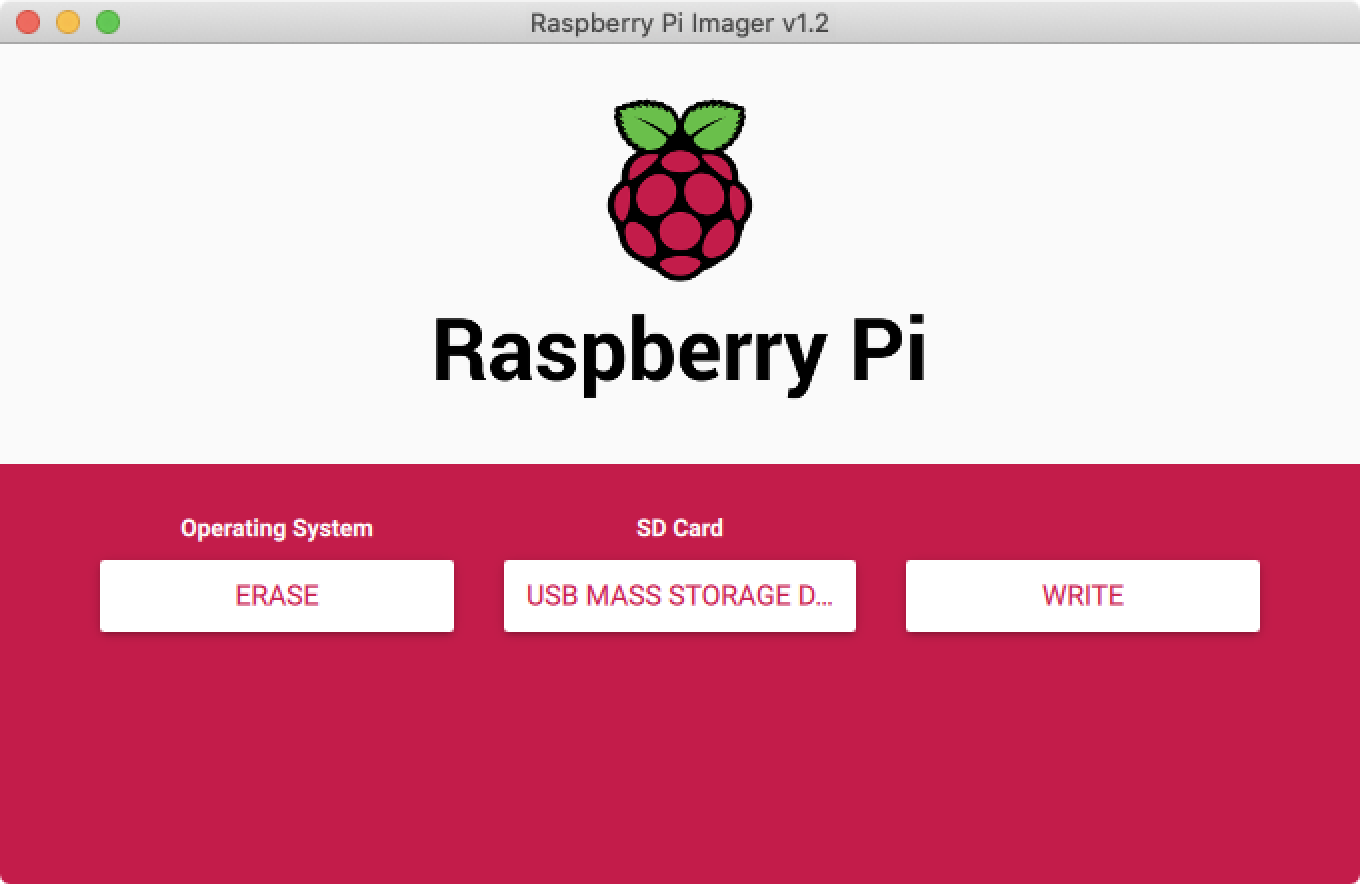
\includegraphics[width=1.0\textwidth]{screenshots/imager-erase.png}
	\caption{Using Raspberry Pi Imager to erase and format a MicroSD card.}
\end{figure}

\begin{figure}[H]
	\centering	
	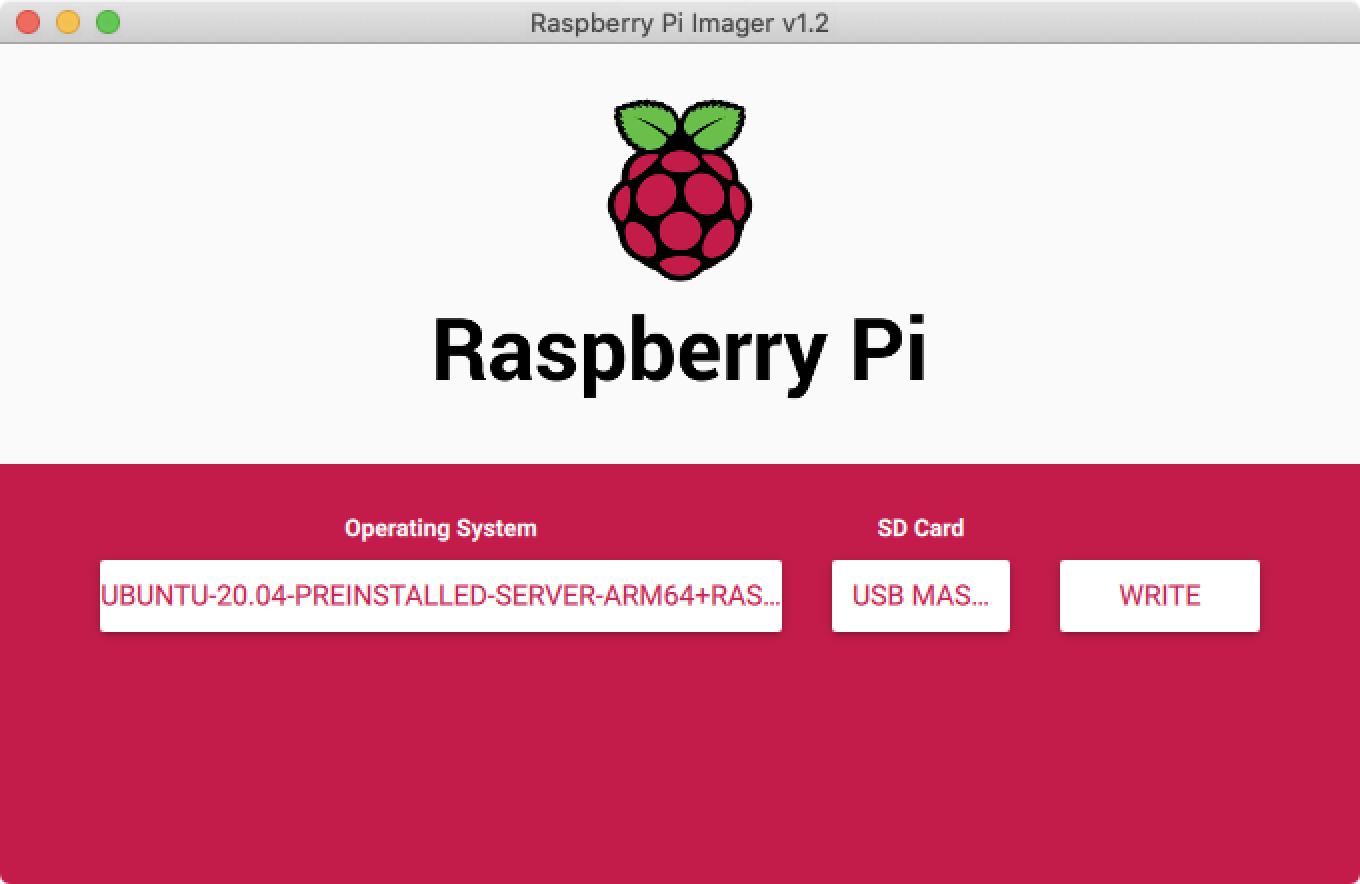
\includegraphics[width=1.0\textwidth]{screenshots/imager-write.png}
	\caption{Using Raspberry Pi Imager to write the server image to a MicroSD card.}
\end{figure}



%
% SECTION
%
\section{Ubuntu Installation}

Having burnt the installation image to each MicroSD card, place the card in each node and plug in the power cable. The \verb|cloud-init| configuration process will now start. Each node will acquire its IP address from the router/firewall, setup system users, update the \verb|apt| cache, upgrade the system, download software packages, set the hostname (based on the IP address), and finally reboot.


%
% SECTION
%
\section{Post-Installation Tasks}


%
% SUB SECTION
%
\subsection{Complete the OpenMPI Password-Less Process}

The user \verb|john|'s public key was installed on each node by \verb|cloud-init|.

It remains to copy the private key to \verb|node1|:

\lstset{style=type}
\begin{lstlisting}
$ scp ~/.ssh/id_rsa node1:~/.ssh
\end{lstlisting}

To complete the process the host keys from \verb|node2| to \verb|node9| need to be imported into the \verb|known_hosts| file of \verb|node1|.

From \verb|macbook|, \verb|ssh| into \verb|node1|:

\lstset{style=type}
\begin{lstlisting}[]
$ ssh node1
\end{lstlisting}

Then from \verb|node1|, \verb|ssh| into \verb|node2| to \verb|node9| in turn, for example:

\lstset{style=type}
\begin{lstlisting}[]
$ ssh node2
\end{lstlisting}


This will generate a message similar to this:

\lstset{style=type}
\begin{lstlisting}[]
The authenticity of host 'node2 (192.168.0.2)' can't be established.
ECDSA key fingerprint is SHA256:5VgsnN2nPvpfbJmALh3aJdOeT/NvDXqN8TCreQyNaFA.
Are you sure you want to continue connecting (yes/no/[fingerprint])?
\end{lstlisting}

Responding \verb|yes| to this this message, imports the \verb|node2| host key into the \verb|~/.ssh/known_hosts| file of \verb|node1|.

Then exit from the connected node:

\lstset{style=type}
\begin{lstlisting}[]
$ exit
\end{lstlisting}

This completes the process.

Subsequent \verb|ssh| access to \verb|node2| to \verb|node9| from \verb|node1| will be done using password-less public key authentication. This is the mechanism that OpenMPI will use.


%
% SUB SECTION
%

\subsection{Uninstall \texttt{unattended-upgrades}}

The \verb|unattended-upgrades| package is installed automatically. This can potentially interfere with long running benchmarks, so it is preferable to uninstall this package from each node. This can be done using Pi Cluster Tools.

From \verb|macbook|:

\lstset{style=type}
\begin{lstlisting}[]
$ ssh node1
$ ~/picluster/tools/do "sudo apt remove unattended-upgrades"
\end{lstlisting}

It is important not to forget to manually upgrade the cluster regularly using Pi Cluster Tools:

\lstset{style=type}
\begin{lstlisting}[]
$ ssh node1
$ ~/picluster/tools/upgrade
\end{lstlisting}



%
% SUB SECTION
%
\subsection{Add Ubuntu Source Repositories}

The Ubuntu source repositories are required to rebuilding the kernel and other Ubuntu packages. These repositories are added as follows:

\lstset{style=type}
\begin{lstlisting}[]
$ ssh node1
$ sudo touch /etc/apt/sources/list.d/picluster.list
\end{lstlisting}

Then add the following to the newly created \verb|picluster.list| file:

\lstset{style=listing}
\begin{lstlisting}[caption=/etc/apt/sources.list.d/picluster.list]
deb-src http://archive.ubuntu.com/ubuntu focal main universe
deb-src http://archive.ubuntu.com/ubuntu focal-updates main universe
\end{lstlisting}

And finally, update the \verb|apt| repository cache:

\lstset{style=type}
\begin{lstlisting}[]
$ sudo apt update
\end{lstlisting}



\subsection{Create a Project Repository}

A project repository on \verb|node1| is required to hold all project software and results. This repository is mirrored with the GitHub project repository.

The project repository is created as follows:

\lstset{style=type}
\begin{lstlisting}[]
$ ssh node1
$ mkdir picluster
$ cd picluster
$ git init
\end{lstlisting}



%
% CHAPTER
%
\chapter{Install High-Performance Linpack (HPL)}

These instructions are derived from the \verb|INSTALL| and \verb|README| files in the \verb|hpl-2.3| top level source directory.

Download and install the latest version of HPL on \verb|node1|:

\lstset{style=type}
\begin{lstlisting}
$ ssh node1
$ cd ~/picluster
$ mkdir hpl
$ cd hpl
$ wget https://www.netlib.org/benchmark/hpl/hpl-2.3.tar.gz
$ gunzip hpl-2.3.tar.gz
$ tar xvf hpl-2.3.tar
$ rm hpl-2.3.tar
$ cd hpl-2.3
\end{lstlisting}

Each computer system requires a specific \verb|Make.picluster| file, which specifies the operating system commands and software package locations required to build HPL. 

Create a generic \verb|Make.picluster| file:

\lstset{style=type}
\begin{lstlisting}
$ cd setup
$ bash make_generic
$ cp Make.UNKNOWN ../Make.picluster
$ cd ..
\end{lstlisting}

Amend \verb|Make.picluster| with the specifics of the Raspberry Pi 4 and Ubuntu 20.04 as follows. The changes below are changes to the generic file created above.

Set the \emph{shell} to use:

\lstset{style=listing}
\begin{lstlisting}[numbers=none]  
SHELL        = /usr/bin/bash
\end{lstlisting}

Set the commands to use (these may vary form operating system to operating system):

\lstset{style=listing}
\begin{lstlisting}[numbers=none]  
CD           = cd
CP           = cp
LN_S         = ln -s
MKDIR        = mkdir -p
RM           = rm -f
TOUCH        = touch
\end{lstlisting}

Set the platform identifier:

\lstset{style=listing}
\begin{lstlisting}[numbers=none]  
ARCH         = picluster
\end{lstlisting}

Set the top level source directory:

\lstset{style=listing}
\begin{lstlisting}[numbers=none]  
TOPdir       = $(HOME)/picluster/hpl/hpl-2.3
\end{lstlisting}

Set the location of the OpenMPI library:

\lstset{style=listing}
\begin{lstlisting}[numbers=none]  
MPdir        = /usr/lib/aarch64-linux-gnu/openmpi
MPinc        = $(MPdir)/include
MPlib        = $(MPdir)/lib/libmpi.so
\end{lstlisting}

Set the location of the BLAS library (Note, this is the location of the Debian \emph{alternatives} \verb|libblas.so.3| library. The actual library that this points to, OpenBLAS or BLIS, is set through the Debian \verb|update-alternatives| command. This can be conveniently done using Pi Cluster Tools.):

\lstset{style=listing}
\begin{lstlisting}[numbers=none]  
LAdir        = /usr/lib/aarch64-linux-gnu
LAinc        =
LAlib        = $(LAdir)/libblas.so.3
\end{lstlisting}

Set the ``Fortran to C'' defintitions, the header directories and libraries: 

\lstset{style=listing}
\begin{lstlisting}[numbers=none]  
F2CDEFS      = -DAdd_ -DF77_INTEGER=int -DStringSunStyle
...
HPL_INCLUDES = -I$(INCdir) -I$(INCdir)/$(ARCH) -I$(MPinc)
HPL_LIBS     = $(HPLlib) $(LAlib) $(MPlib)
...
HPL_DEFS     = $(F2CDEFS) $(HPL_OPTS) $(HPL_INCLUDES)
\end{lstlisting}

And finally, set the compiler, linker and optimisation flags:

\lstset{style=listing}
\begin{lstlisting}[numbers=none]  
CC           = mpicc
CCNOOPT      = $(HPL_DEFS)
CCFLAGS      = $(HPL_DEFS) -O3 -march=armv8-a -mtune=cortex-a72
...
LINKER       = $(CC)
LINKFLAGS    = $(CCFLAGS)
...
ARCHIVER     = ar
ARFLAGS      = r
RANLIB       = echo
\end{lstlisting}

Build HPL:

\lstset{style=type}
\begin{lstlisting}
$ make arch=picluster   
\end{lstlisting}

This creates the executable \verb|xhpl| and input file \verb|HPL.dat| in the \verb|bin/picluster| directory.

The \verb|xhpl| executable has to exist in the same location on each node, so copy \verb|xhpl| to \verb|node2| to \verb|node8| (only \verb|xhpl|, and not \verb|HPL.dat|):

\lstset{style=type}
\begin{lstlisting}
$ cd bin/picluster
$ ~/picluster/tools/do "mkdir -p picluster/hpl/hpl-2.3/bin/picluster"
$ scp xhpl node2:~picluster/hpl/hpl-2.3/bin/picluster
$ scp xhpl node3:~picluster/hpl/hpl-2.3/bin/picluster
$ scp xhpl node4:~picluster/hpl/hpl-2.3/bin/picluster
$ scp xhpl node5:~picluster/hpl/hpl-2.3/bin/picluster
$ scp xhpl node6:~picluster/hpl/hpl-2.3/bin/picluster
$ scp xhpl node7:~picluster/hpl/hpl-2.3/bin/picluster
$ scp xhpl node8:~picluster/hpl/hpl-2.3/bin/picluster
\end{lstlisting}


%
% CHAPTER
%
\chapter{Install HPC Challenge (HPCC)}

These instructions are derived from the README.txt file in the top level directory of the HPCC source code.

It is assumed that HPL has previously been installed, and a HPL build file \verb|Make.picluster| has already been created. This file is copied to the HPCC build directory. See Chapter 8 for the instructions on how to install HPL.

Download and install the latest version of HPCC on \verb|node1|:

\lstset{style=type}
\begin{lstlisting}
$ ssh node1
$ cd ~/picluster
$ mkdir hpcc
$ cd hpcc
$ wget http://icl.cs.utk.edu/projectsfiles/hpcc/download/hpcc-1.5.0.tar.gz
$ gunzip hpcc-1.5.0.tar.gz
$ tar xvf hpcc-1.5.0.tar
$ rm hpcc-1.5.0.tar
$ cd hpcc-1.5.0
\end{lstlisting}

Copy the HPL build script \verb|Make.picluster| to the HPCC \verb|hpl| directory:

\lstset{style=type}
\begin{lstlisting}
$ cd hpl
$ cp ~/picluster/hpl/hpl-2.3/Make.picluster .
\end{lstlisting}

Make the following changes to \verb|Make.picluster|. These differ from the HPL build instructions:

Change the \verb|TOPdir| variable:

\lstset{style=hack}
\begin{lstlisting}[caption=Make.picluster]
TOPdir = ../../..
\end{lstlisting}

Add the \verb|math| library explicitly:

\lstset{style=hack}
\begin{lstlisting}[caption=Make.picluster]
LAlib = $(LAdir)/libblas.so.3 -lm
\end{lstlisting}

Add the constant \verb|OMPI_OMIT_MPI1_COMPAT_DECLS| to \verb|CCFLAGS|, otherwise the compilation will fail:

\lstset{style=hack}
\begin{lstlisting}[caption=Make.picluster]
CCFLAGS = $(HPL_DEFS) -O3 -march=armv8-a -mtune=cortex-a72 -DOMPI_OMIT_MPI1_COMPAT_DECLS
\end{lstlisting}

Move back up into the top level directory:

\lstset{style=type}
\begin{lstlisting}
$ cd ..
\end{lstlisting}

Build HPCC:

\lstset{style=type}
\begin{lstlisting}
$ make arch=picluster
\end{lstlisting}

Copy the \verb|hpcc| executable to the compute nodes:

\lstset{style=type}
\begin{lstlisting}
$ ~/picluster/tools/do "mkdir -p ~/picluster/hpcc/hpcc-1.5.0"
$ scp hpcc node2:~/picluster/hpcc/hpcc-1.5.0
$ scp hpcc node3:~/picluster/hpcc/hpcc-1.5.0
$ scp hpcc node4:~/picluster/hpcc/hpcc-1.5.0
$ scp hpcc node5:~/picluster/hpcc/hpcc-1.5.0
$ scp hpcc node6:~/picluster/hpcc/hpcc-1.5.0
$ scp hpcc node7:~/picluster/hpcc/hpcc-1.5.0
$ scp hpcc node8:~/picluster/hpcc/hpcc-1.5.0
\end{lstlisting}

Create the input file \verb|hpccinf.txt|:

\lstset{style=type}
\begin{lstlisting}
$ cp _hpccinf.txt hpccinf.txt
\end{lstlisting}

The input file is amended as necessary for each benchmark run, as per the HPL input file.

After each benchmark run the results will be in the output file \verb|hpccoutf.txt|.



%
% CHAPTER
%
\chapter{Install High Performance Conjugate Gradients (HPCG)}

These instructions are derived from the INSTALL and QUICKSTART files in the HPCG 3.1 top-level source directory.

\lstset{style=hack}
\begin{lstlisting}
The main build difference between HPCG and HPL is that HPCG can be built as either a single-threaded serial program, or a multi-threaded OpenMP program. It is not the BLAS library which is either single or multi-threaded. In fact, HPCG does not use a BLAS library. To investigate the performance of HPCG in either single-threaded or multi-threaded versions requires building two HPCG programs.
\end{lstlisting}

Download and install the latest version of HPCG on \verb|node1|:

\lstset{style=type}
\begin{lstlisting}
$ ssh node1
$ cd ~/picluster
$ mkdir hpcg
$ cd hpcg
$ wget http://www.hpcg-benchmark.org/downloads/hpcg-3.1.tar.gz
$ gunzip hpcg-3.1.tar.gz
$ tar xvf hpcg-3.1.tar
$ rm hpcg-3.1.tar
$ cd hpcg-3.1
\end{lstlisting}


%
% SECTION
%
\section{Serial HPCG}

Create a \verb|Make.picluster_serial| file for the serial build:

\lstset{style=type}
\begin{lstlisting}
$ cp setup/Make.Linux_serial setup/Make.picluster_serial
\end{lstlisting}

Amend \verb|setup/Make.picluster_serial| as follows.

Set the shell:

\lstset{style=listing}
\begin{lstlisting}[numbers=none]
SHELL = /usr/bin/bash
\end{lstlisting}

Set the top level directory:

\lstset{style=listing}
\begin{lstlisting}[numbers=none]
TOPdir = $(HOME)/picluster/hpcg/hpcg-3.1
\end{lstlisting}

Set the OpenMPI package location:

\lstset{style=listing}
\begin{lstlisting}[numbers=none]
MPdir = /usr/lib/aarch64-linux-gnu/openmpi
MPinc = $(MPdir)/include
MPlib = $(MPdir)/lib/libmpi.so
\end{lstlisting}

Include the OpenMPI header files and library:

\lstset{style=listing}
\begin{lstlisting}[numbers=none]
HPCG_INCLUDES = -I$(INCdir) -I$(INCdir)/$(arch) -I$(MPinc)
HPCG_LIBS     = $(MPlib)
\end{lstlisting}

Ensure HPCG is built without OpenMP support:

\lstset{style=listing}
\begin{lstlisting}[numbers=none]
HPCG_OPTS = -DHPCG_NO_OPENMP
\end{lstlisting}

Set C++ compiler flags:

\lstset{style=listing}
\begin{lstlisting}[numbers=none]
CXX      = mpic++
CXXFLAGS = $(HPCG_DEFS) -O3 -march=armv8-a -mtune=cortex-a72
\end{lstlisting}

Build HPCG:

\lstset{style=type}
\begin{lstlisting}[numbers=none]
$ mkdir build_serial
$ cd build_serial
$ ../configure picluster_serial
$ make
\end{lstlisting}

This creates the serial version of the \verb|xhpcg| executable and the \verb|hpcg.dat| input file in the \verb|build_serial/bin| directory.


%
% SECTION
%
\section{OpenMP HPCG}

Create a \verb|Make.picluster_openmp| file for the OpenMP build:

\lstset{style=type}
\begin{lstlisting}
$ cp setup/Make.Linux_serial setup/Make.picluster_openmp
\end{lstlisting}

Amend \verb|setup/Make.picluster_openmp| as per \verb|setup/Make.pcluster_serial|, with the exceptions of not disabling OpenMP, i.e. leave HPCG\_OPTS blank, and adding \verb|-fopenmp| to the compiler flags:

\lstset{style=listing}
\begin{lstlisting}[numbers=none]
HPCG_OPTS = 
\end{lstlisting}

\lstset{style=listing}
\begin{lstlisting}[numbers=none]
CXXFLAGS = $(HPCG_DEFS) -O3 -march=armv8-a -mtune=cortex-a72 -fopenmp
\end{lstlisting}

This is a bug fix for \verb|src/ComputeResidual.cpp| line 56. Add the variable \verb|n| to the shared variables list of \verb|omp parallel| clause, otherwise a compiler error is generated:

\lstset{style=hack}
\begin{lstlisting}[numbers=none]
#pragma omp parallel default(none) shared(n, local_residual, v1v, v2v)
\end{lstlisting}


Build HPCG:

\lstset{style=type}
\begin{lstlisting}[numbers=none]
$ mkdir build_openmp
$ cd build_openmp
$ ../configure picluster_openmp
$ make
\end{lstlisting}

This creates the OpenMP version of the \verb|xhpcg| executable and the \verb|hpcg.dat| input file in the \verb|build_openmp/bin| directory.


%
% CHAPTER
%
\chapter{Ubuntu Kernel Build Procedure}

This procedure is derived from the Ubuntu Wiki BuildYourOwnKernel document...

Make sure you have made the source code repositories available as per...

Create a kernel build directory with the correct directory permissions to prevent source download warnings. 

\lstset{style=type}
\begin{lstlisting}
$ ssh node1
$ mkdir -p ~/picluster/build/kernel
$ sudo chown _apt:root ~/picluster/build/kernel
$ cd ~/picluster/build/kernel
\end{lstlisting}

Install the kernel build dependencies...

\lstset{style=type}
\begin{lstlisting}
$ sudo apt-get build-dep linux linux-image-$(uname -r)
\end{lstlisting}

Download the kernel source...

\lstset{style=type}
\begin{lstlisting}
$ sudo apt-get source linux-image-$(uname -r)
$ cd linux-raspi-5.4.0
\end{lstlisting}

This bit is a fix for the subsequent \verb|editconfigs| step of the build procedure...

\lstset{style=type}
\begin{lstlisting}
$ cd debian.raspi/etc
$ sudo cp kernelconfig kernelconfig.original
$ sudo vim kernelconfig
\end{lstlisting}

And make the following change...

\lstset{style=listing}
\begin{lstlisting}[caption=diff kernelconfig kernelconfig.original, numbers=none]
5c5
< 	archs="arm64"
---
> 	archs="armhf arm64"
\end{lstlisting}

Then move back up to the kernel source top level directory...

\lstset{style=type}
\begin{lstlisting}
$ cd ../..
\end{lstlisting}

Prepare the build scripts...

\lstset{style=type}
\begin{lstlisting}
$ sudo chmod a+x debian/rules
$ sudo chmod a+x debian/scripts/*
$ sudo chmod a+x debian/scripts/misc/*
\end{lstlisting}

SOURCE CHANGES AND/OR verb|editconfigs| AT THIS POINT

\lstset{style=type}
\begin{lstlisting}
$ sudo apt install libncurses-dev
$ sudo LANG=C fakeroot debian/rules clean
$ sudo LANG=C fakeroot debian/rules editconfigs
\end{lstlisting}

Tweak the kernel name for identification...

\lstset{style=type}
\begin{lstlisting}
$ cd debian.raspi
$ sudo cp changelog changelog.original
$ sudo vim changelog
\end{lstlisting}

And make the following change, where \verb|+picluster0| is our kernel identifier...

\lstset{style=listing}
\begin{lstlisting}[caption=diff changelog changelog.original, numbers=none]
1c1
< linux-raspi (5.4.0-1015.15+picluster0) focal; urgency=medium
---
> linux-raspi (5.4.0-1015.15) focal; urgency=medium
\end{lstlisting}

Move up to the top level kernel source directory...

\lstset{style=type}
\begin{lstlisting}
$ cd ..
\end{lstlisting}

And build the kernel...

\lstset{style=type}
\begin{lstlisting}
$ sudo LANG=C fakeroot debian/rules clean
$ sudo LANG=C fakeroot debian/rules binary-arch
cd ..
\end{lstlisting}

Install the new kernel...

\lstset{style=type}
\begin{lstlisting}
$ sudo dpkg -i linux*picluster0*.deb
$ sudo shutdown -r now
\end{lstlisting}

Another build procedure fix...

After each kernel build delete the \verb|linux-libc-dev| directory...

\lstset{style=type}
\begin{lstlisting}
$ cd ~/picluster/build/kernel/linux-raspi-5.4.0/debian
$ rm -rf linux-libc-dev
$ cd ..
\end{lstlisting}


%
% CHAPTER
%
\chapter{Build Kernel with No Pre-Emption Scheduler}


%
% CHAPTER
%
\chapter{Build Kernel with Jumbo Frames Support}

Standard MTU is 1500 bytes...

Maximum payload size is 1472 bytes...

NB of 184 (x 8 bytes for Double Precision) = 1472 bytes...

NB $>$ 184 $=>$ packet fragmentation $=>$ reduced network efficiency...

This causes drop of in performance???...

Max MTU on Raspberry Pi 4 Model B is set at build time to 1500...

Not configurable above 1500...

TODO: EXAMPLE OF ERROR MSG...

Need to build the kernel with higher MTU...


Make the required changes to the source... as per REFERENCE

\begin{verbatim}
    cd linux-raspi-5.4.0 

    sudo vim include/linux/if_vlan.h...
        #define VLAN_ETH_DATA_LEN   9000
        #define VLAN_ETH_FRAME_LEN  9018
    
    sudo vim include/uapi/linux/if_ether.h...
        #define ETH_DATA_LEN        9000
        #define ETH_FRAME_LEN       9014
    
    sudo vim drivers/net/ethernet/broadcom/genet/bcmgenet.c...
        #define RX_BUF_LENGTH       10240
\end{verbatim}

Add a Jumbo Frames identifier, "+jf", to the new kernel name...

\begin{verbatim}
    sudo vim debian.raspi/changelog...
        linux (5.4.0-1013.13+jf) focal; urgency=medium
        
\end{verbatim}


%
% CHAPTER
%
\chapter{Rebuild OpenBLAS}

\lstset{style=type}
\begin{lstlisting}
$ ssh node1
$ mkdir -p build/openblas
$ chown -R _apt:root build
$ cd build/openblas
$ sudo apt-get source openblas
$ sudo apt-get build-dep openblas
$ cd openblas-0.3.8+ds
\end{lstlisting}


Edit cpuid\_arm64.c...

\lstset{style=type}
\begin{lstlisting}
$ sudo cp cpuid_arm64.c cpuid_arm64.c.original
$ sudo vim cpuid_arm64.c
\end{lstlisting}


\lstset{style=type}
\begin{lstlisting}
$ diff cpuid_arm64.c cpuid_arm64.c.original
\end{lstlisting}

\lstset{style=type}
\begin{lstlisting}
275c275
<       printf("#define L2_SIZE 1048576\n");
---
>       printf("#define L2_SIZE 524288\n");
278c278
<       printf("#define DTB_DEFAULT_ENTRIES 32\n");
---
>       printf("#define DTB_DEFAULT_ENTRIES 64\n");
\end{lstlisting}


And, then following the instructions in debian/README.Debian

\lstset{style=type}
\begin{lstlisting}
$ DEB_BUILD_OPTIONS=custom dpkg-buildpackage -uc -b
\end{lstlisting}

Once the build is complete..

\lstset{style=type}
\begin{lstlisting}
cd ..
$ sudo apt remove libopenblas0-serial
$ sudo dpkg -i libopenblas0-serial\_0.3.8+ds-1\_arm64.deb
\end{lstlisting}

Ensure the correct BLAS library is being used...

\lstset{style=type}
\begin{lstlisting}
$ sudo update-alternatives --config libblas.so.3-aarch64-linux-gnu
\end{lstlisting}

copy to other nodes
remove old...
install new...

If more than one BLAS library is installed, check update-alternatives!!!

ssh node2 .. node8
\lstset{style=type}
\begin{lstlisting}
$ ssh node2 sudo apt remove libblas0-serial
$ scp libopenblas0-serial\_0.3.8+ds-1\_arm64.deb node2:~
$ ssh sudo dpkg -i libopenblas0-serial\_0.3.8+ds-1\_arm64.deb
$ ssh sudo update-alternatives --config libblas.so.3-aarch64-linux-gnu
\end{lstlisting}


%
% CHAPTER
%
\chapter{Rebuild BLIS}

\lstset{style=type}
\begin{lstlisting}
$ ssh node1
$ mkdir -p picluster/build/blis
$ cd picluster/build/blis
$ apt-get source blis
$ sudo apt-get build-dep blis
$ cd blis-0.6.1
\end{lstlisting}


%
% CHAPTER
%

\chapter{Build OpenMPI from Source}

Do all of this on node1...

\lstset{style=type}
\begin{lstlisting}
$ ssh node1
\end{lstlisting}

We want to avoid collisions with multiple OpenMPI installations, so remove original installed version...

\lstset{style=type}
\begin{lstlisting}
$ sudo apt remove openmpi-common
$ sudo apt remove openmpi-bin
$ sudo apt autoremove 
\end{lstlisting}

OpenMPI requires the libevent-dev package...

\lstset{style=type}
\begin{lstlisting}
$ sudo apt install libevent-dev
\end{lstlisting}

Create a build directory, and download and, and and following BLAH, BLAH build OpenMPI...

\lstset{style=type}
\begin{lstlisting}
$ mkdir -p ~/picluster/build/openmpi
$ cd ~/picluster/build/openmpi
$ wget https://download.open-mpi.org/release/open-mpi/v4.0/openmpi-4.0.4.tar.gz
$ gunzip openmpi-4.0.4.tar.gz
$ tar xvf openmpi-4.0.4.tar
$ rm openmpi-4.0.4.tar
$ cd openmpi-4.0.4
$ mkdir build
$ cd build
$ ../configure CFLAGS="-O3 -march=armv8-a -mtune=cortex=a72"
$ make all
$ sudo make install
$ sudo ldconfig
\end{lstlisting}

OpenMPI will installed to /usr/local

EXTRACT FROM HPL.dat


TODO: HOW TO COPY TO ALL NODES!


%
% CHAPTER
%
\chapter{Aerin Cluster Tools}

\lstinputlisting[caption=picluster/tools/upgrade, numbers=left, backgroundcolor=\color{LightSkyBlue}]{picluster/tools/upgrade}
\lstinputlisting[caption=picluster/tools/reboot, numbers=left, backgroundcolor=\color{LightSkyBlue}]{picluster/tools/reboot}
\lstinputlisting[caption=picluster/tools/shutdown, numbers=left, backgroundcolor=\color{LightSkyBlue}]{picluster/tools/shutdown}
\lstinputlisting[caption=picluster/tools/libblas-query, numbers=left, backgroundcolor=\color{LightSkyBlue}]{picluster/tools/libblas-query}
\lstinputlisting[caption=picluster/tools/libblas-set, numbers=left, backgroundcolor=\color{LightSkyBlue}]{picluster/tools/libblas-set}


%
% CHAPTER
%

\chapter{Arm Performance Libraries}

\textcolor{red}{This does not work, yet! HPL will compile and link to Arm Performance Libraries, but raises an illegal instruction error at runtime.}

\textcolor{red}{At the time of writing, Arm Performance Libraries release 20.2.0 requires a minimum Instruction Set Architecture (ISA) of armv8.1-a. Unfortunately, the Raspberry Pi's Cortex-A72 ISA is armv8.0-a. An Arm representative has indicated on the Arm HPC Forum that the next release of the libraries will support the armv8.0-a ISA.}

\textcolor{red}{This Chapter is included for future reference.}

The Arm Performance Libraries website states:

"Arm Performance Libraries provides optimised standard core math libraries for high-performance computing applications on Arm processors. This free version of the libraries provides optimised libraries for Arm® Neoverse™ N1-based Armv8 AArch64 implementations that are compatible with various versions of GCC. You do not require a license for this version of the libraries."

To install Arm Performance Libraries, firstly downloaded Arm Performance Libraries 20.2.0 with GCC 9.3 for Ubuntu 16.04+ from the Arm website.

Then follow these instructions.

\lstset{style=type}
\begin{lstlisting}
$ ssh node1
\end{lstlisting}

Install the required \verb|environment_modules| package.

\lstset{style=type}
\begin{lstlisting}
$ sudo apt install environment-modules
\end{lstlisting}

Then extract and install Arm Performance Libraries.

The default installation directory is /opt/arm.

\lstset{style=type}
\begin{lstlisting}
$ mkdir ~/picluster/armpl
$ cd ~/picluster/armpl
$ tar xvf arm-performance-libraries_20.2_Ubuntu-16.04_gcc-9.3.tar
$ rm arm-performance-libraries_20.2_Ubuntu-16.04_gcc-9.3.tar
$ sudo ./arm-performance-libraries_20.2_Ubuntu-16.04.sh
\end{lstlisting}

Copy the \verb|Make.picluster| configuration file.

\lstset{style=type}
\begin{lstlisting}
$ cd ~/picluster/hpl/hpl-2.3
$ cp Make.picluster Make.picluster-armpl
\end{lstlisting}

Make the following changes to \verb|Make.picluster-armpl|.

\lstset{style=listing}
\begin{lstlisting}[caption=Make.picluster-armpl, numbers=none]
LAdir        = /opt/arm/armpl_20.2_gcc-9.3
LAinc        =
LAlib        = -L$(LAdir)/lib -larmpl -lgfortran -lamath -lm
\end{lstlisting}

Build HPL.

\lstset{style=type}
\begin{lstlisting}
$ make arch=picluster-armpl
\end{lstlisting}


%
% THE END
%
\end{document}
